\documentclass[11pt,a4paper]{article}
% Latin Modern with T1 encoding when available; otherwise Computer Modern.
\IfFileExists{lmodern.sty}{\usepackage[T1]{fontenc}\usepackage{lmodern}}{}
\usepackage[utf8]{inputenc}
\usepackage[margin=27mm,headheight=14pt]{geometry}
\usepackage{amsmath,amssymb,amsthm,mathtools}
\usepackage{microtype}
\usepackage{array,booktabs,tabularx,xltabular,needspace,float}
\usepackage{fancyhdr}
\usepackage[dvipsnames]{xcolor}
\usepackage{tikz}
\usetikzlibrary{arrows.meta,positioning,fit,backgrounds}
\usepackage{url}
\usepackage[unicode]{hyperref}
\hypersetup{colorlinks=true,
  linkcolor=NavyBlue!75!black,citecolor=ForestGreen!70!black,urlcolor=NavyBlue!75!black}
\usepackage{bookmark}
% Lean identifiers: typewriter, breakable at dots, slashes and underscores.
\DeclareUrlCommand\lean{\urlstyle{tt}}
% A slightly more compact table of contents, with room for two-digit numbers.
\makeatletter
\renewcommand*\l@section[2]{%
  \ifnum \c@tocdepth >\z@
    \addpenalty\@secpenalty
    \addvspace{0.4em \@plus\p@}%
    \setlength\@tempdima{1.9em}%
    \begingroup
      \parindent \z@ \rightskip \@pnumwidth
      \parfillskip -\@pnumwidth
      \leavevmode \bfseries
      \advance\leftskip\@tempdima
      \hskip -\leftskip
      #1\nobreak\hfil
      \nobreak\hb@xt@\@pnumwidth{\hss #2}%
      \kern-\p@\kern\p@
      \par
    \endgroup
  \fi}
\makeatother
\numberwithin{equation}{section}
\newtheorem{theorem}{Theorem}[section]
\newtheorem{lemma}[theorem]{Lemma}
\newtheorem{proposition}[theorem]{Proposition}
\newtheorem{corollary}[theorem]{Corollary}
\theoremstyle{definition}
\newtheorem{definition}[theorem]{Definition}
\theoremstyle{remark}
\newtheorem{remark}[theorem]{Remark}
\newcommand{\F}{\mathbb F_2}
\newcommand{\Fav}{\mathsf F}
\newcommand{\cZ}{\mathcal Z}
\newcommand{\Om}{\Omega}
\newcommand{\E}{\mathbb E}
\newcommand{\Prob}{\mathbb P}
\newcommand{\cc}{\operatorname{comp}}
\newcommand{\supp}{\operatorname{supp}}
\newcommand{\dist}{\operatorname{dist}}
\newcommand{\tr}{\operatorname{tr}}
\newcommand{\rank}{\operatorname{rank}}
\newcommand{\lstar}{\log_*}
\newcommand{\eps}{\varepsilon}
\newcommand{\secsign}{\ensuremath{\S}}
% Run-in headings for the steps of long proofs.
\newcommand{\proofstep}[1]{\par\addvspace{\medskipamount}\noindent\textbf{#1}\enspace\ignorespaces}
\newcommand{\ee}{\mathrm e}
\newcommand{\ind}{\mathbf 1}
\newcommand{\ceil}[1]{\left\lceil#1\right\rceil}
\newcommand{\floor}[1]{\left\lfloor#1\right\rfloor}
\DeclareMathOperator{\Var}{Var}
\setlength{\emergencystretch}{2em}
\widowpenalty=10000 \clubpenalty=10000 \displaywidowpenalty=10000
\linespread{1.035}
\allowdisplaybreaks[2]
\pagestyle{fancy}
\fancyhf{}
\fancyhead[L]{\footnotesize The minimum number of edges in a pancyclic graph}
\fancyhead[R]{\footnotesize\itshape\nouppercase{\leftmark}}
\renewcommand{\sectionmark}[1]{\markboth{\thesection\enspace #1}{}}
\fancyfoot[C]{\thepage}
\renewcommand{\headrulewidth}{0.3pt}
\hypersetup{pdftitle={The minimum number of edges in a pancyclic graph},pdfauthor={KNT},pdfsubject={The sharp asymptotic bound for the minimum number of edges in a pancyclic graph}}
\title{\LARGE\bfseries The minimum number of edges\\[4pt] in a pancyclic graph}
\newcommand{\paperauthors}{KNT}
\author{\paperauthors}
\date{September 2026}
\begin{document}
\maketitle
\begin{abstract}
For $n\ge3$, let $h(n)$ be the least $h$ for which some graph with $n$ vertices and $n+h$ edges contains a cycle of every length from $3$ to $n$. Bondy stated in 1971 that $\log_2(n-1)-1\le h(n)\le\log_2n+\log_*n+O(1)$, and whether the lower bound can be raised to match is Erd\H{o}s Problem \#1016. We prove that $h(n)=\log_2 n+\log_*n+O(1)$, where $\log_*$ counts iterated binary logarithms.

The lower bound comes from a near-halving inequality for the normalized cycle-length capacity of graphs: one exponential level of cycle rank multiplies it by at most $1/2+1/R$, up to an additive error, and these departures from exact halving are summable. The graph-theoretic core of this inequality does not mention cycle lengths. In a connected graph of very large cycle rank, a uniformly random even edge set restricted to the complement of a small active subgraph with few components is a linear forest with probability at most $1/2+1/R$. The proof uses a bound on the cut information shared by three disjoint regions, a stretched-exponential forest estimate obtained from nonbacktracking walks and conditional factorial moments, and a cut-tree descent with a signed count of exterior components. A binary-shortcut construction gives $h(n)\le\floor{\log_2n}+\log_*n+1$ for every $n\ge3$. A complete proof of the main theorem has been formalized in Lean~4.

\medskip
\noindent\textit{MSC 2020:} 05C38 (primary); 05C35, 05C50, 60C05 (secondary).\\
\textit{Keywords:} pancyclic graphs, cycle lengths, cycle space, nonbacktracking walks, Erd\H{o}s problems, formal verification.
\end{abstract}
\newpage
\setcounter{tocdepth}{2}
{\linespread{1}\selectfont\tableofcontents}
\newpage
\section{Introduction}\label{sec:intro}
A finite simple graph on $n$ vertices is \emph{pancyclic} if it contains a simple cycle of each length $3,4,\ldots,n$. Define
\[
 h(n)=\min\{|E(G)|-n:G\text{ is a pancyclic graph on }n\text{ vertices}\}.
\]
Cycle lengths always count edges of the graph itself. For $x\ge1$, let $\lstar x$ be the least nonnegative integer $j$ such that $j$ successive applications of $\log_2$ take $x$ to a value at most one. Other common stopping conventions change $\lstar$ by at most an absolute constant.

\begin{theorem}\label{thm:main}
There are absolute constants $A_-,A_+$ such that, for every integer $n\ge3$,
\[
 \log_2n+\lstar n-A_-\le h(n)\le\log_2n+\lstar n+A_+.
\]
In particular, $h(n)=\log_2n+\lstar n+O(1)$. One may take $A_+=1$.
\end{theorem}

The extremal question goes back to Bondy \cite{Bondy}. Writing $m(n)=n+h(n)$ for the minimum number of edges, he stated without proof that
\[
 n-1+\log_2(n-1)\le m(n)\le n+\log_2n+H(n)+O(1),
\]
where $H(n)$ is the least number of iterated binary logarithms taking $n$ below $2$. Thus $\log_2(n-1)-1\le h(n)\le\log_2n+\lstar n+O(1)$. The lower bound is the cycle-counting argument recalled in Section~\ref{sec:why-logstar}; a written proof was given by Griffin \cite{Griffin}, who also computed $m(n)$ exactly for small $n$. On the constructive side, Sridharan \cite{Sridharan} gave pancyclic graphs with $O(\log n)$ added chords. The sharp upper construction is discussed in the monograph of George, Khodkar and Wallis \cite{GKW}, and the same binary-shortcut mechanism underlies the sparse pancyclic subgraphs of random graphs found by Alon and Krivelevich \cite{AK}.

Whether the lower bound can be raised to $\log_2n+\lstar n-O(1)$, or at least whether $h(n)-\log_2n\to\infty$, is Problem~\#1016 in the collection of Erd\H{o}s problems \cite{ErdosProblems}. Theorem~\ref{thm:main} answers both questions affirmatively. It determines $h(n)$ up to an absolute additive constant, although not its exact value for each $n$. The upper bound, with $A_+=1$, is proved in Section~\ref{sec:upper}; the rest of the paper proves the lower bound.

\subsection{Why an iterated logarithm appears}\label{sec:why-logstar}
A connected graph with $n+h$ edges has a binary cycle space of dimension $h+1$, and therefore at most $2^{h+1}-1$ simple cycles. A pancyclic graph needs at least $n-2$ of them, one of each length, which gives the classical bound $h\ge\log_2(n-1)-1$. This count sees only how many cycles there are. It does not see that their lengths must fill an entire interval, and it is this additional rigidity that produces the term $\lstar n$.

To measure it, let $I(r)$ be the largest $L$ such that some graph of cycle rank at most $r$ contains cycles of all lengths $3,\ldots,L$, and consider the normalized tail
\[
 \Phi(R)=\sup_{r\ge R}\frac{I(r)-2}{2^r}.
\]
The counting bound says only that $\Phi\le1$. The central estimate of the paper is the recurrence
\begin{equation}\label{eq:intro-recurrence}
 \Phi(2^{CR^4})\le\left(\frac12+\frac1R\right)\Phi(R)+2^{2-R}
 \qquad(R\ge R_0),
\end{equation}
with absolute integers $C,R_0$. Passing from the scale $R$ to the scale $2^{CR^4}$ costs one exponential level of rank and nearly halves the normalized capacity. Along the scales $R_{j+1}=2^{CR_j^4}$, the relative errors $1/R_j$ are summable, and so are the additive errors even after they are amplified by $2^j$. After $j$ steps the capacity is therefore at most a constant multiple of $2^{-j}$, rather than merely $q^j$ for some fixed $q>1/2$. Reaching rank $r$ takes $\lstar r+O(1)$ steps, so a pancyclic graph on $n$ vertices of rank $r$ satisfies
\[
 n-2\le2^r\,\Phi(r)\le O\bigl(2^{\,r-\lstar r}\bigr).
\]
This is the lower bound of Theorem~\ref{thm:main}; the details are in Section~\ref{sec:contraction}.

\subsection{A complement theorem independent of pancyclicity}\label{sec:complement-intro}
The graph-theoretic part of the proof can be stated without any assumption on cycle lengths. For a graph $G$, let $\cZ(G)$ be its binary cycle space: the family of edge sets in which every vertex has even degree. It is a vector space over $\F$ of dimension $\beta(G)=|E(G)|-|V(G)|+\cc(G)$, the \emph{cycle rank}, where $\cc$ counts connected components. A uniformly random element of $\cZ(G)$ is a uniformly random even edge set. An edge is \emph{active} if it lies on a cycle of $G$, or equivalently if it is not a bridge; each active edge belongs to the random even edge set with probability $1/2$, and every other edge never does. A \emph{linear forest} is an acyclic edge set of maximum degree at most two. For a set $M$ of edges, put
\[
 \ell_G(M)=\Prob_{x\in\cZ(G)}[x\cap M\text{ is a linear forest}].
\]
In the next statement, the vertices and components of an edge subgraph $W$ are counted on its edge support.

\begin{theorem}[Linear forests outside a small active subgraph]\label{thm:complement}
There are absolute integers $C\ge8$ and $R_0\ge5$ such that the following holds for every integer $R\ge R_0$. Let $G$ be a connected finite simple graph of cycle rank
\[
 r=\beta(G)\ge 2^{CR^4}.
\]
Let $W$ be a nonempty edge subgraph all of whose edges are active in $G$. With $m=|E(W)|$, assume
\[
 |V(W)|\le m,\qquad m+1\le 2^{4R},\qquad \cc(W)<5R.
\]
Then, for $M=E(G)\setminus E(W)$,
\begin{equation}\label{eq:intro-complement}
 \ell_G(M)\le\frac12+\frac1R.
\end{equation}
\end{theorem}

Both a size bound and a component bound are assumed, and the component bound does not follow from the size bound: $W$ may have exponentially many edges in $R$, but only $O(R)$ components. In the pancyclic application, $W$ is the union of chosen cycles of the lengths $3,\ldots,2^{2R}+1$. Its edges are automatically active, it has no vertex of degree one, and a competitiveness condition on the cycle-length count supplies the bound $\cc(W)<5R$ (Lemma~\ref{lem:screen}). Apart from this, the proof of Theorem~\ref{thm:complement}, completed in Section~\ref{sec:complement-proof}, makes no use of cycle lengths.

\subsection{Two exact interfaces}
The proof relates two kinds of information: which cycle lengths occur in a graph, which is numerical, and which edge sets are compatible with its parity constraints, which is probabilistic. Both interfaces between them are kept exact.

On the numerical side, we count \emph{distinct lengths of linear forests}, rather than the forests themselves. A cycle that crosses an edge partition $W\cup M$, where $W$ consists of one chosen cycle of each short length, restricts to a linear forest on each side, and the two pieces have the same set of odd-degree vertices. We keep the exact space of such common boundaries (Lemma~\ref{lem:composition}). A probability then bounds one factor of the resulting numerical expression; it does not replace the capacity itself.

On the probabilistic side, we use the uniform measure on the \emph{complete} cycle space of the graph. The components outside a chosen region impose separate parity equations on its boundary. Passing from the average over all even boundary demands to the actual marginal law therefore costs a factor $2^{c-1}$ when there are $c$ exterior components (Lemma~\ref{lem:core-transfer}). A useful region must have not only many vertices but also few exterior components. This is why the cut-tree argument of Section~\ref{sec:descent} and the reduction of Section~\ref{sec:cleanup} keep track of the components outside a region, even after vertices have been discarded.

\subsection{Organization of the proof}\label{sec:organization}
Figure~\ref{fig:structure} shows how the parts fit together. Section~\ref{sec:capacity} introduces numerical capacity and bounds the rank of a short-cycle witness. Section~\ref{sec:graphical} proves a covariance bound for graphical cut spaces, which is used both in the descent and in the reduction. Sections~\ref{sec:analytic-basics}--\ref{sec:forest-decay} prove the stretched-exponential forest estimate, Theorem~\ref{thm:forest-decay}, for mildly expanding graphs of maximum degree three. Section~\ref{sec:descent} combines it with a cut-tree descent to handle regions that need not expand. Section~\ref{sec:cleanup} reduces a general graph to such a region while preserving the original witness and the probability law. Section~\ref{sec:contraction} proves Theorem~\ref{thm:complement} and then derives and iterates \eqref{eq:intro-recurrence}. Section~\ref{sec:upper} gives the upper construction, and Appendix~\ref{app:lean} describes the formalization.

\begin{figure}[H]
\centering
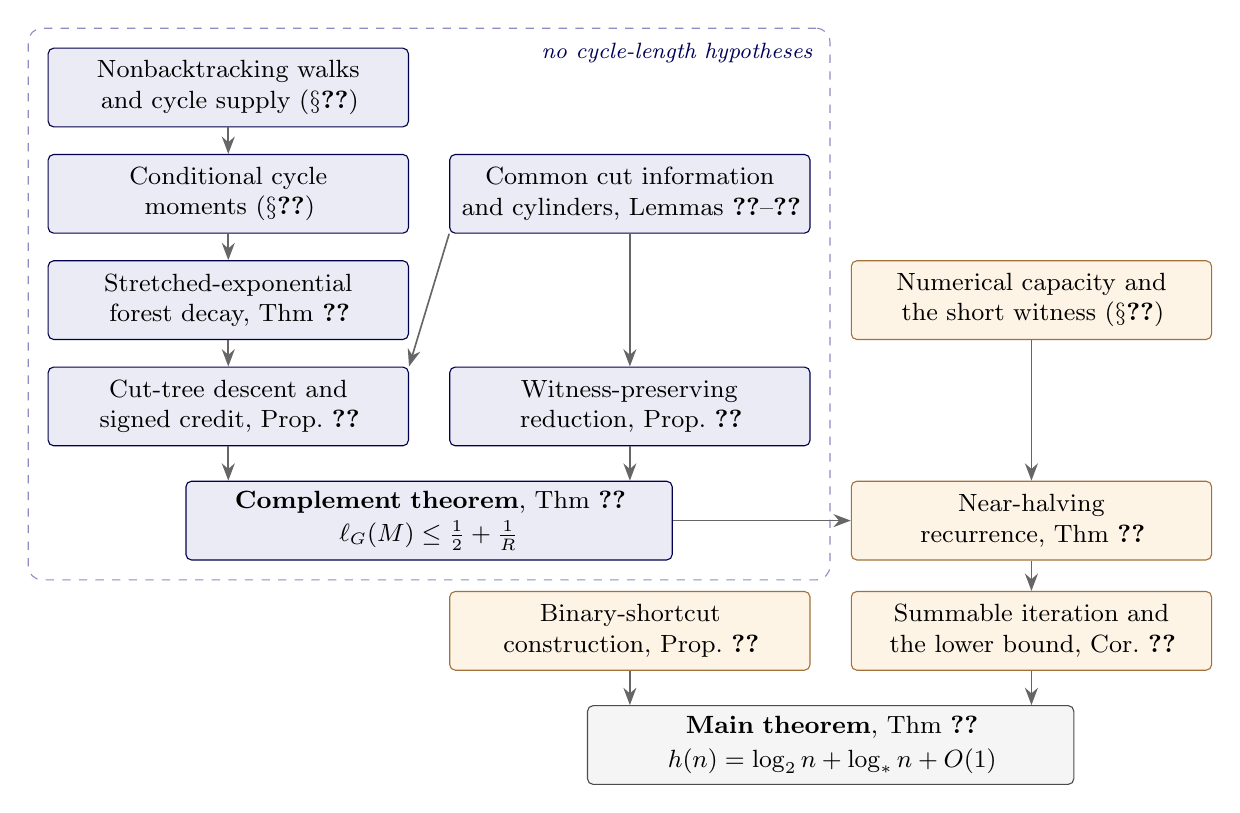
\begin{tikzpicture}[
  font=\small,
  box/.style={draw=#1!60!black, fill=#1!8, rounded corners=2pt, align=center,
              text width=4.4cm, minimum height=10mm, inner sep=2.5pt,
              execute at begin node={\hyphenpenalty=10000\exhyphenpenalty=10000}},
  box/.default=NavyBlue,
  arr/.style={-{Stealth[length=2.2mm]}, semithick, draw=black!60}]
 % graph-theoretic part (no cycle-length hypotheses)
 \node[box] (nb) at (0,0)     {Nonbacktracking walks and cycle supply (\secsign\ref{sec:analytic-basics})};
 \node[box] (cm) at (0,-1.35)  {Conditional cycle moments (\secsign\ref{sec:conditional})};
 \node[box] (fd) at (0,-2.7)  {Stretched-exponential forest decay, Thm~\ref{thm:forest-decay}};
 \node[box] (de) at (0,-4.05)  {Cut-tree descent and signed credit, Prop.~\ref{prop:descent}};
 \node[box] (gr) at (5.1,-1.35) {Common cut information and cylinders, Lemmas~\ref{lem:triple}--\ref{lem:many-regions}};
 \node[box] (re) at (5.1,-4.05) {Witness-preserving reduction, Prop.~\ref{prop:cleanup}};
 \node[box, text width=6.0cm] (ct) at (2.55,-5.5)
      {\textbf{Complement theorem}, Thm~\ref{thm:complement}\\[1pt] \mbox{$\ell_G(M)\le\tfrac12+\tfrac1R$}};
 % numerical part
 \node[box=BurntOrange] (cap) at (10.2,-2.7) {Numerical capacity and the short witness (\secsign\ref{sec:capacity})};
 \node[box=BurntOrange] (rec) at (10.2,-5.5) {Near-halving recurrence, Thm~\ref{thm:recurrence}};
 \node[box=BurntOrange] (low) at (10.2,-6.9) {Summable iteration and the lower bound, Cor.~\ref{cor:lower}};
 \node[box=BurntOrange] (up) at (5.1,-6.9) {Binary-shortcut construction, Prop.~\ref{prop:upper}};
 \node[box=Gray, text width=6.0cm] (main) at (7.65,-8.35)
      {\textbf{Main theorem}, Thm~\ref{thm:main}\\[1pt] \mbox{$h(n)=\log_2n+\log_*n+O(1)$}};
 \draw[arr] (nb) -- (cm);
 \draw[arr] (cm) -- (fd);
 \draw[arr] (fd) -- (de);
 \draw[arr] (gr) -- (re);
 \draw[arr] (gr.south west) -- (de.north east);
 \draw[arr] (de.south) -- (de.south|-ct.north);
 \draw[arr] (re.south) -- (re.south|-ct.north);
 \draw[arr] (ct) -- (rec);
 \draw[arr] (cap) -- (rec);
 \draw[arr] (rec) -- (low);
 \draw[arr] (low.south) -- (low.south|-main.north);
 \draw[arr] (up.south) -- (up.south|-main.north);
 \begin{scope}[on background layer]
  \node[draw=NavyBlue!45, dashed, rounded corners=5pt, inner sep=7pt,
        fit=(nb) (gr) (ct) (de) (re)] (frame) {};
  \node[font=\footnotesize\itshape, text=NavyBlue!70!black, anchor=north east]
        at ([xshift=-3pt,yshift=-2pt]frame.north east) {no cycle-length hypotheses};
 \end{scope}
\end{tikzpicture}
\caption{Logical structure of the proof. Everything inside the dashed frame concerns general graphs and uniform even edge sets; cycle lengths enter only through Section~\ref{sec:capacity} and the recurrence of Section~\ref{sec:contraction}.}
\label{fig:structure}
\end{figure}

\subsection{Formal verification}\label{sec:lean}
A complete proof of Theorem~\ref{thm:main}, including the analytic estimates of Sections~\ref{sec:analytic-basics}--\ref{sec:forest-decay}, the reduction of Section~\ref{sec:cleanup} and the construction of Section~\ref{sec:upper}, has been formalized in Lean~4 \cite{Lean4} using the Mathlib library \cite{Mathlib}. The development is available at
\begin{center}
\url{https://github.com/JWKNT/erdos1016}.
\end{center}
The version described here is commit \texttt{9ca8b0d}, which uses Lean v4.19.0 and a pinned Mathlib revision. It consists of about $83{,}000$ lines in $495$ Lean modules, including the root import module.

The formal statement is deliberately elementary, so that it can be compared with Theorem~\ref{thm:main} without reading the proof. Cycles are Mathlib's \lean{SimpleGraph.Walk.IsCycle}; $h(n)$ is the infimum of $|E(G)|-n$ over pancyclic simple graphs $G$ on the vertex type \texttt{Fin n}; and $\lstar n$ is the least $j$ with $n\le T(j)$, where $T(0)=1$ and $T(j+1)=2^{T(j)}$, which agrees with the convention above. The theorem \lean{Erdos1016.mainTheorem} asserts that there are real constants $A_-,A_+$ such that
\[
 \log_2n+\lstar n-A_-\le h(n)\le\log_2n+\lstar n+A_+\qquad(n\ge3).
\]
A companion theorem proves the same bound when $h(n)$ is defined instead as the minimum edge count minus $n$, computed in the integers.

The repository's verification script rebuilds every module from source, checks the fully expanded statements, confirms that the main theorem carries no hypotheses, and rejects any axiom other than Lean's standard \texttt{propext}, \texttt{Classical.choice} and \texttt{Quot.sound}. The sources contain no \texttt{sorry}, no \texttt{native\_decide} and no added axioms. Commit \texttt{9ca8b0d} passed this fresh verification in the repository's continuous integration (GitHub Actions run \href{https://github.com/JWKNT/erdos1016/actions/runs/36026578423}{36026578423}), whose verification record is attached to the run. Appendix~\ref{app:lean} lists the Lean counterparts of the main steps.

\subsection{Conventions and parity facts}\label{sec:parity}
Graphs are finite and undirected, and the graphs in Theorem~\ref{thm:main} are simple. The auxiliary multigraphs of Sections~\ref{sec:descent} and~\ref{sec:cleanup} may have parallel edges and loops, which remain distinguished; a loop contributes two to the degree, and a loop or a pair of parallel edges counts as a cycle. An edge subgraph is taken on its edge support, without artificial isolated vertices. Isolated vertices do not affect the cycle rank.

We identify edge subsets with vectors over $\F$, so that addition is symmetric difference. The boundary $\partial x$ of an edge set $x$ is its set of odd-degree vertices, and we write
\[
 \cZ(G)=\{x\subseteq E(G):\partial x=\varnothing\},
 \qquad
 \Om_T(G)=\{x\subseteq E(G):\partial x=T\}.
\]
A spanning forest shows that $\dim\cZ(G)=\beta(G)$. More explicitly, prescribe the non-tree coordinates arbitrarily and determine the tree coordinates by successively removing leaves; the last equation in each component is satisfied exactly when that component meets $T$ in an even number of vertices. Consequently every nonempty $\Om_T(G)$ is a translate of $\cZ(G)$ and has exactly $2^{\beta(G)}$ elements. The same holds for the auxiliary multigraphs.

All probabilities below are uniform on the specified finite space. The image of a uniform vector under a linear map is uniform on the image, since every fiber is a coset of the kernel, and the same holds on a nonempty affine space. We use this repeatedly, always with the \emph{whole} image and all of its fibers.

A forest is an acyclic edge set. The only even forest is the empty set, since a nonempty finite forest has a leaf. Every simple cycle is a nonzero element of $\cZ(G)$, so
\begin{equation}\label{eq:cycle-count}
 C(G)\le2^{\beta(G)}-1,
\end{equation}
where $C(G)$ is the number of simple cycles, counted as edge sets. We write $\lambda(G)$ for the number of distinct lengths among them. Logarithms are binary unless written $\ln$.

A constant is \emph{absolute} if it depends neither on the graph nor on the scale under consideration. When a statement is made for fixed parameters $c,B$, its constants and its threshold for ``sufficiently large'' may depend on $c,B$, but are uniform over the corresponding class of graphs. This matters in the analytic estimate, whose parameters are fixed once and for all before the scale $R$ varies. We keep the growth of every scale-dependent bound explicit, but do not assign numerical values to absolute constants whose size plays no role.

\subsection{Notation used across the proof}
The table collects the symbols that are used in more than one section; each is defined where it first appears. They distinguish numerical length counts, which are always normalized by an actual cycle rank, from physical probabilities under a uniform even edge set.
\begin{center}
\small
\renewcommand{\arraystretch}{1.12}
\begin{tabularx}{\linewidth}{@{}>{$}l<{$}Xr@{}}
\toprule
\text{Symbol} & Meaning & Where \\
\midrule
\beta(G),\ \cZ(G),\ \Om_T(G) & Cycle rank; binary cycle space; edge sets with odd-vertex set $T$ & \secsign\ref{sec:parity} \\
C(G),\ \lambda(G) & Number of simple cycles; number of distinct cycle lengths & \secsign\ref{sec:parity} \\
\ell_G(M) & Probability that a uniform even edge set is a linear forest on $M$ & \secsign\ref{sec:complement-intro} \\
I(r),\ f(r),\ \Phi(R) & Longest initial interval at rank ${}\le r$; its normalization; normalized tail & \secsign\ref{sec:capacity} \\
\nu_F(T),\ a(F),\ \alpha(L) & Linear-forest length count; local capacity; prefix capacity & \secsign\ref{sec:capacity} \\
U,\ \sigma_G(M) & Common-boundary image of a partition; numerical coefficient & \secsign\ref{sec:capacity} \\
P_\Gamma(F),\ P_\Gamma(J) & Probability that the restriction to $F$ (or to $E(J)$) is a forest & \secsign\ref{sec:graphical} \\
q_R,\ \mathcal N_R(d),\ \mathfrak n_d & Target $\frac12+\frac1R$; number of cyclic regions forcing it; its fixed-cut constant & \secsign\ref{sec:graphical} \\
\iota(H),\ \Fav(H) & Edge expansion; forest probability averaged over even port demands & \secsign\ref{sec:analytic-basics} \\
I_C,\ a_C & Component event of a cycle $C$; its weight $2^{-|C|}$ & \secsign\secsign\ref{sec:analytic-basics}--\ref{sec:conditional} \\
k,\ t_0,\ \Lambda,\ d_* & Moment order; first trace length; retained weight; conditional load & \secsign\secsign\ref{sec:conditional}--\ref{sec:forest-decay} \\
K,\ K_{\mathcal U} & A two-core; the two-core after conditioning on $\mathcal U$ & \secsign\ref{sec:conditional}, \secsign\ref{sec:descent} \\
b(J),\ c(J),\ \Psi(J) & Boundary size; exterior component count; deficit potential & \secsign\ref{sec:descent} \\
T_0(c),\ D_0 & Analytic stopping size; small-leaf cut bound & \secsign\ref{sec:descent} \\
\mathcal A_R & Bound for the attachments of the protected set & \secsign\ref{sec:cleanup} \\
\bottomrule
\end{tabularx}
\end{center}
A few letters are reused with a local meaning. In Sections~\ref{sec:analytic-basics}--\ref{sec:forest-decay}, $W$ denotes a connected protected vertex set containing the apex, $L$ a length horizon and $D$ a girth parameter; elsewhere $W$ is the short-cycle witness and $L=2^{2R}+1$. In Section~\ref{sec:descent} the leaves of the cut tree are also denoted by $L$. The mean of a random variable is denoted by $\mu$ only inside local second-moment calculations.

\section{Numerical capacity and a short witness}\label{sec:capacity}
\subsection{The capacity definitions}
A lower bound on edges is a bound on how efficiently a graph of a given cycle rank can realize an initial interval of lengths. We first measure this efficiency globally, then introduce a local quantity that behaves well when edges are restricted.

For an integer $r\ge0$, let $I(r)$ be the largest $L\ge2$ for which a finite simple graph of cycle rank at most $r$ contains all lengths $3,\ldots,L$. Empty coverage is permitted, so $I(0)=2$. Equation~\eqref{eq:cycle-count} gives $I(r)\le2^r+1$, and the maximum exists because the attainable endpoints form a nonempty bounded set of integers. Put
\[
 f(r)=\frac{I(r)-2}{2^r},\qquad \Phi(R)=\sup_{r\ge R}f(r).
\]
Disconnected realizers are allowed. Identifying one vertex from each component makes them connected without changing any cycle lengths or their rank. Adding triangles by one-vertex unions can then raise the actual rank to a prescribed larger integer without shortening the initial interval. Whenever we do this, we apply a theorem afresh to the resulting graph; no boundary law is transported through the identification.

The restriction of a cycle to a proper part of its edges is a linear forest. Once its odd vertices are specified, only the possible total lengths of that forest matter for completing cycle lengths. This motivates the following local definition.

For a graph $F$ and a vertex demand $T$, let $\mathcal L_F(T)$ be the set of edge counts of linear forests in $\Om_T(F)$, and define
\[
 \nu_F(T)=|\mathcal L_F(T)|,\qquad
 a(F)=2^{-\beta(F)}\max_T\nu_F(T),
\]
with infeasible demands contributing zero. Finally, set
\[
 \alpha(L)=\sup\{a(F):F\text{ contains every cycle length }3,\ldots,L\}.
\]
We have $\nu_F(\varnothing)=1$ and $0<a(F)\le1$. The function $\alpha$ is nonincreasing. A one-vertex union of cycles of lengths $3,\ldots,R+2$ has rank $R$, so
\begin{equation}\label{eq:calibration}
 R2^{-R}\le\Phi(R)\le1\qquad(R\ge1).
\end{equation}

\subsection{Restriction and the finite bridge}
\begin{lemma}[Capacity under restriction]\label{lem:monotonicity}
If $H$ is an edge subgraph of $F$, then $a(F)\le a(H)$. Also, if $H\subseteq G$, then
\begin{equation}\label{eq:oneshot}
 \lambda(G)\le\bigl(2^{\beta(G)-\beta(H)}-1\bigr)
                   \max_T\nu_H(T)+\lambda(H).
\end{equation}
\end{lemma}
\begin{proof}
Restrict a feasible complete parity class on $F$ to $E(F)\setminus E(H)$. The restriction kernel is $\cZ(H)$, so there are $2^{\beta(F)-\beta(H)}$ outside words. In a fixed outside word, the inner odd set is fixed and the inner fiber is complete. A linear forest restricts to a linear forest. Its possible lengths therefore lie in a translate of $\mathcal L_H(T)$ for the corresponding demand. A union bound over the outside words proves
\[
 \max_T\nu_F(T)\le2^{\beta(F)-\beta(H)}\max_T\nu_H(T),
\]
and hence the first assertion.

For a simple cycle in $G$ whose outside restriction relative to $H$ is nonzero, the restriction to $H$ is a linear forest. Each such outside word contributes at most $\max_T\nu_H(T)$ distinct total lengths. The zero outside word contributes only cycles contained in $H$. This proves \eqref{eq:oneshot}.
\end{proof}

\begin{lemma}[A finite bridge]\label{lem:bridge}
For every integer $R\ge5$,
\begin{equation}\label{eq:bridge}
 \alpha(2^{2R}+1)\le\Phi(R)+2^{1-R}.
\end{equation}
\end{lemma}
\begin{proof}
Starting with the empty subgraph of a graph $F$, repeatedly adjoin one cycle of the least missing length, until the desired initial interval is covered. At preceding actual rank $s$, the new cycle has length at most $I(s)+1$. It introduces a new edge: otherwise that length was already present. Its vector is therefore outside the old cycle space, so rank increases by at least one. If the terminal support $H$ has rank $p$, the preceding ranks are a subset of $\{0,\ldots,p-1\}$, even when some rank increments exceed one. Hence
\begin{equation}\label{eq:greedy}
 |E(H)|\le\sum_{s=0}^{p-1}(I(s)+1).
\end{equation}

Let $\phi=\Phi(R)$. Below $R$, use $I(s)+1\le2^s+2$; at and above $R$, use $I(s)+1\le\phi2^s+3$. For $p\ge R$ this gives
\[
 |E(H)|+1\le\phi2^p+(1-\phi)2^R+3p-R
                  \le\phi2^p+2^R+3p.
\]
Now let $F$ cover $3,\ldots,L$, where $L=2^{2R}+1$, and run this procedure inside $F$ until that interval is covered. Equation~\eqref{eq:cycle-count} implies $p\ge2R$. Lemma~\ref{lem:monotonicity} and the bound $\nu_H(T)\le|E(H)|+1$ yield
\[
 a(F)\le\phi+\frac{2^R+3p}{2^p}.
\]
The last fraction decreases for integers $p\ge2R$. Since $6R\le2^R$ for $R\ge5$, it is at most $2^{1-R}$. Taking the supremum over $F$ proves the lemma.
\end{proof}

\subsection{The actual common-boundary image}
Let $E(G)=E(A)\mathbin{\dot\cup}E(M)$ be an actual edge partition. Write $r=\beta(G)$, $r_A=\beta(A)$, $r_M=\beta(M)$, and let
\[
 U=\operatorname{im}\bigl(\cZ(G)\longrightarrow\F^{V(G)},\ 
                       x\longmapsto\partial(x\cap E(A))\bigr),
 \qquad d=\dim U.
\]
Since $x$ is even, $x\cap E(M)$ has the same boundary as $x\cap E(A)$. The kernel of this map is $\cZ(A)\oplus\cZ(M)$, so
\begin{equation}\label{eq:actual-rank}
 r=r_A+r_M+d.
\end{equation}
For each $T\in U$, the two restrictions range over exactly
$\Om_T(A)\times\Om_T(M)$. In particular, both factors are complete, with respective sizes $2^{r_A}$ and $2^{r_M}$. The number $d$ need not equal the interface size minus one: additional component equations can lower it.

Define the numerical coefficient
\begin{equation}\label{eq:sigma}
 \sigma_G(M)=2^{-r_M-d}\sum_{T\in U\setminus\{\varnothing\}}\nu_M(T),
\end{equation}
and recall the physical probability
\[
 \ell_G(M)=\Prob_{x\in\cZ(G)}[x\cap E(M)\text{ is a linear forest}].
\]

\begin{lemma}[Numerical composition]\label{lem:composition}
For the preceding partition,
\begin{align}
 \frac{\lambda(G)}{2^r}
 &\le a(A)\sigma_G(M)+2^{-r_A-d}+2^{-r_M-d},\label{eq:composition}\\
 \sigma_G(M)&\le\ell_G(M)-2^{-r_M-d}.\label{eq:sigma-physical}
\end{align}
\end{lemma}
\begin{proof}
A simple cycle using both parts restricts to a nonempty proper linear forest in each. Its common odd set is nonempty, because an even forest is empty. Its length belongs to
$\mathcal L_A(T)+\mathcal L_M(T)$ for some nonzero $T\in U$. Consequently
\[
 \lambda(G)\le\lambda(A)+\lambda(M)+
       \sum_{T\in U\setminus\{\varnothing\}}\nu_A(T)\nu_M(T).
\]
Use $\nu_A(T)\le2^{r_A}a(A)$, bound the pure-side cycle counts by \eqref{eq:cycle-count}, and divide by \eqref{eq:actual-rank}. Discarding the resulting negative term proves \eqref{eq:composition}.

Let $\mathrm{LF}_M(T)$ be the number of physical linear forests in $\Om_T(M)$. Complete-fiber uniformity gives
\[
 \ell_G(M)=2^{-r_M-d}\sum_{T\in U}\mathrm{LF}_M(T).
\]
For every $T$, $\nu_M(T)\le\mathrm{LF}_M(T)$, and $\mathrm{LF}_M(\varnothing)=1$. Subtract the latter term to obtain \eqref{eq:sigma-physical}.
\end{proof}

\subsection{The rank of a short-cycle witness}
Fix $R\ge5$, put $L=2^{2R}+1$ and $\phi=\Phi(R)$, and suppose $G$ contains all lengths $3,\ldots,L$. Choose one actual cycle of each of these lengths \emph{before} any extraction, and let $W$ be their union. Let $m=|E(W)|$ and $r_W=\beta(W)$. Then
\begin{equation}\label{eq:witness-size}
 m\le\frac{L(L+1)}2-3,\qquad m+1\le2^{4R},\qquad |V(W)|\le m.
\end{equation}
The second bound follows on substituting $L$: the first upper bound plus one is
$2^{4R-1}+3\cdot2^{2R-1}-1\le2^{4R}$.

A graph whose normalized number of cycle lengths is below $\Phi(R)/2$ already satisfies the inequality we are aiming for (see the proof of Theorem~\ref{thm:recurrence}), so only the following graphs need attention. We call a graph $G$ \emph{competitive at scale $R$} when
\begin{equation}\label{eq:competitive}
 \lambda(G)2^{-\beta(G)}\ge\phi/2.
\end{equation}
\begin{lemma}[Witness rank bound]\label{lem:screen}
If $G$ is competitive and $r=\beta(G)\ge5R+2$, every selected witness $W$ as above satisfies
\begin{equation}\label{eq:witness-screen}
 2R\le r_W<5R,\qquad \cc(W)\le r_W<5R.
\end{equation}
For $M=G\setminus E(W)$, one also has $\beta(M)\ge r-m$.
\end{lemma}
\begin{proof}
Lemma~\ref{lem:monotonicity}, $\nu_W(T)\le m+1$ and $\lambda(W)\le m$ give
\[
 \lambda(G)2^{-r}\le(m+1)2^{-r_W}+m2^{-r}.
\]
If $r_W\ge5R$, \eqref{eq:witness-size} and $r\ge5R+2$ make this at most
$(5/4)2^{-R}<(R/2)2^{-R}\le\phi/2$, contradicting competitiveness. Since $W$ contains $L-2$ distinct lengths, \eqref{eq:cycle-count} gives $r_W\ge2R$. Every component of the union $W$ contains a cycle, whence $\cc(W)\le r_W$. Finally, deleting $m$ coordinates can lower a vector-space dimension by at most $m$, giving $\beta(M)\ge r-m$.
\end{proof}

The distinction between $m$ and $\cc(W)$ is essential: the witness may have exponentially many edges in $R$, but it has only $O(R)$ components. The edge count will be paid for by removing rank, while the component count will control the exterior of the region constructed in Section~\ref{sec:cleanup}.

\section{Common cut information and many cyclic regions}\label{sec:graphical}
This section isolates a property of graphical parity spaces: three disjoint regions cannot share two independent pieces of cut information (Lemma~\ref{lem:triple}). Two regions can share much more, so an argument based on pairwise independence would fail. The resulting second-moment bound, Lemma~\ref{lem:cylinders}, shows that many disjoint cyclic regions with small cuts force the forest probability down to nearly one half (Lemma~\ref{lem:many-regions}). These estimates are used in the descent of Section~\ref{sec:descent} and in two steps of the reduction of Section~\ref{sec:cleanup}.

\subsection{A triple-intersection bound}
For a vertex $v$ of a connected loopless multigraph $Q$, let $L_v$ be the span in $\cZ(Q)^*$ of the coordinate functionals of the edges incident to $v$. Equivalently,
\[
 L_v=\{\text{linear functionals on }\cZ(Q)\text{ vanishing on }\cZ(Q-v)\}.
\]
The equality follows because the kernel of restriction to that star is exactly the zero extension of $\cZ(Q-v)$.

\begin{lemma}[Graphical common information]\label{lem:triple}
For three distinct vertices $u,v,w$,
\[
 \dim(L_u\cap L_v\cap L_w)\le1.
\]
The same assertion holds for the cut-coordinate spaces of three pairwise vertex-disjoint connected regions in a connected multigraph.
\end{lemma}
\begin{proof}
For fixed $u,v$, list the following links: each individual $uv$ edge, and each component of $Q-\{u,v\}$ having an attachment to both $u$ and $v$. Let there be $t$ links. Given $x\in\cZ(Q)$, a direct-edge link has bit $x_e$; a component link has bit equal to the parity of the selected edges from $u$ into that component. Summing the parity equations in the component shows that this equals the parity from $v$. Components attached to only one of $u,v$ contribute even parity there. Thus the link bits have even total parity and define a map
\[
 \varphi:\cZ(Q)\longrightarrow
 E_t=\{z\in\F^t:\textstyle\sum_i z_i=0\}.
\]
This map is onto. Choose a simple $u$--$v$ path within each component link; the union of any two distinct link paths realizes the corresponding pair of unit bits. Such pairs span $E_t$.

We claim
\begin{equation}\label{eq:link-kernel}
 \ker\varphi=\cZ(Q-u)+\cZ(Q-v).
\end{equation}
The right-hand side clearly has zero link bits. Conversely, a kernel word has zero direct $uv$ coordinates and even attachment parity at both ends of every component link, so it splits into even words on the separate components with their attachments to $u,v$. In a component meeting both, choose a spanning tree of the component and one attachment edge to each of $u,v$. A fundamental cycle arising from another $u$ attachment avoids $v$; one from another $v$ attachment avoids $u$; an internal chord avoids both. These cycles span the even space of that attached component. Components meeting only one of the two vertices are simpler. This proves \eqref{eq:link-kernel}.

A functional in $L_u\cap L_v$ can therefore be written as coefficients $(a_1,\ldots,a_t)$ on the link bits, modulo the all-one coefficient vector. The third vertex $w$ belongs to at most one component link. Any pair of the other links is realized by a cycle avoiding $w$. If the functional is also in $L_w$, it vanishes on every such cycle. All coefficients except possibly the one exceptional coefficient must be equal. Modulo the all-one vector, at most one parameter remains. The cases $t\le1$ are immediate.

For disjoint connected regions, contract each whole region to a vertex and delete its internal edges. Restriction from the original cycle space onto the quotient cycle space is surjective: the even total demand at each contracted vertex can be filled inside the corresponding connected region. Pullback embeds the quotient dual and identifies each marked star space with the original cut-coordinate space. The vertex assertion applies. Loops elsewhere can be discarded for this purpose; their independent coordinates occur in no cut.
\end{proof}

\subsection{A second moment with its common mode retained}
\begin{lemma}[Graphical cylinder bound]\label{lem:cylinders}
Let $L_1,\ldots,L_t$ be subspaces of the dual of a finite binary vector space, of dimensions at most $d$, with $\dim(L_i\cap L_j\cap L_k)\le1$ whenever $i,j,k$ are pairwise distinct. For each $i$, fix a feasible assignment on $L_i$, and let $A_i$ be the corresponding affine cylinder in the uniform homogeneous space. Put
\[
 p_i=\Prob(A_i)=2^{-\dim L_i},\qquad Y=\sum_i\ind_{A_i},\qquad \mu=\E Y.
\]
Then
\begin{equation}\label{eq:second-moment}
 \E Y^2\le2\mu^2+(1+2^{2d})\mu.
\end{equation}
\end{lemma}
\begin{proof}
Two assignments are either incompatible on $L_i\cap L_j$, giving zero joint probability, or
\[
 \Prob(A_i\cap A_j)=2^{\dim(L_i\cap L_j)}p_ip_j.
\]
Call a pair exceptional if its intersection has dimension at least two. For fixed $i$, choose a two-dimensional plane in each exceptional intersection. The same plane cannot be used for two different partners: it would lie in a triple intersection. The number of planes is less than the number $2^{2d}$ of ordered pairs of vectors in $L_i$. Thus there are at most $2^{2d}$ exceptional partners of $i$.

For nonexceptional ordered pairs, use $\Prob(A_i\cap A_j)\le2p_ip_j$. For exceptional partners of $i$, use $\Prob(A_i\cap A_j)\le p_i$. The diagonal contributes $\mu$. Summing proves \eqref{eq:second-moment}.
\end{proof}

The factor two is not an error term: a single common parity bit can correlate arbitrarily many events. The exceptional-pair term accounts for the possible larger pairwise intersections.

\subsection{Many zero cuts give a near-half forest bound}
For an edge set $F\subseteq E(\Gamma)$, write
\[
 P_\Gamma(F)=\Prob_{x\in\cZ(\Gamma)}[x\cap F\text{ is a forest}].
\]
A \emph{region} is a set of vertices, identified with the subgraph it induces, and it is \emph{cyclic} if that subgraph contains a cycle. For a region $J$, abbreviate $P_\Gamma(E(J))$ to $P_\Gamma(J)$.

For integers $R\ge5$ and $d\ge0$, define
\begin{equation}\label{eq:moving-count}
 q_R=\frac12+\frac1R,\qquad a_R=\ceil{\log_2(4R)},\qquad
 \mathcal N_R(d)=8R\,2^d(1+2^{2d}+a_R).
\end{equation}
Notice that $a_R\le R$ for $R\ge5$.

\begin{lemma}[Many cyclic regions]\label{lem:many-regions}
Suppose a connected graph $\Gamma$ contains $t\ge\mathcal N_R(d)$ pairwise vertex-disjoint connected cyclic regions $J_1,\ldots,J_t$, each with at most $d$ outgoing edges in $\Gamma$. Then
\[
 P_\Gamma\left(\bigcup_i E(J_i)\right)\le\frac12+\frac1{2R}<q_R.
\]
Adjacency between different regions is permitted.
\end{lemma}
\begin{proof}
Let $A_i$ be the event that no edge of the cut of $J_i$ is selected, and let $Z=\sum_i\ind_{A_i}$. Each $A_i$ is a cylinder over the cut-coordinate space of $J_i$, which has dimension at most $d$. Lemmas~\ref{lem:triple} and \ref{lem:cylinders} give
\[
 \mu=\E Z\ge t2^{-d},\qquad
 \E Z^2\le2\mu^2+\chi_d\mu,\qquad \chi_d=1+2^{2d}.
\]
If $t\ge \mathcal N_R(d)$, then $\mu\ge8R(\chi_d+a_R)$. Since
$\E[Z\ind_{Z<a_R}]\le a_R$, Cauchy--Schwarz gives
\[
 \Prob(Z\ge a_R)\ge\frac{(\mu-a_R)^2}{2\mu^2+\chi_d\mu}
 \ge\frac{(1-x)^2}{2+x}\ge\frac12-2x,
 \qquad x=\frac1{8R}.
\]
The last inequality follows by multiplying through by $2+x$: the difference is $\tfrac32x+3x^2\ge0$.

Reveal \emph{all} edges outside the union of the internal edge sets, including every cut edge and every edge between two regions. In any feasible complete outside word, the remaining choices are a Cartesian product of complete parity classes on the regions. If $A_i$ occurs, the class on $J_i$ is $\cZ(J_i)$, and its only forest is empty. Its conditional forest probability is $2^{-\beta(J_i)}\le1/2$. In every other region use the bound one. It follows that
\begin{equation}\label{eq:conditional-product}
 P_\Gamma\left(\bigcup_i E(J_i)\right)\le\E[2^{-Z}].
\end{equation}
This multiplies internal fibers after complete conditioning, not the zero-cut events themselves. As $2^{-a_R}\le1/(4R)$,
\[
 \E[2^{-Z}]\le1-\Prob(Z\ge a_R)+2^{-a_R}
 \le\frac12+\frac1{2R}.
\]
\end{proof}


For later use, the dependence on $R$ in this threshold can be separated from the dependence on the cut bound. For every fixed integer $d\ge0$, define
\begin{equation}\label{eq:fixed-cut-count}
 \mathfrak n_d=8\,2^d(2+2^{2d}).
 \qquad\text{Then}\qquad
 \mathcal N_R(d)\le \mathfrak n_d R^2\quad(R\ge5).
\end{equation}
Indeed, $a_R\le R$ and $1+2^{2d}+R\le(2+2^{2d})R$. The constant $\mathfrak n_d$ may be large, but when $d$ is fixed the required number of regions grows only quadratically in $R$.

\section{Nonbacktracking walks and cycle supply}\label{sec:analytic-basics}
The next three sections estimate the probability that an even edge set has an acyclic restriction to a region of low boundary size. Expansion prevents small deleted sets from separating off too much of the graph. Nonbacktracking walks then provide a weighted supply of cycles, and the conditional moment argument converts that supply into a forest-probability bound.

\subsection{Expansion and the one-apex completion}
For a connected graph $H$, let
\[
 \iota(H)=\min_{\varnothing\ne S\subsetneq V(H)}
       \frac{|\delta_H(S)|}{\min\{|S|,|H|-|S|\}},\qquad \iota(K_1)=\infty.
\]
Here $|H|=|V(H)|$. Suppose $H$ is simple, connected, and has degrees two or three, with $b\ge1$ degree-two vertices, called ports. Define
\begin{equation}\label{eq:boundary-average}
 \Fav(H)=2^{-(b-1)}\sum_{\substack{T\subseteq B\\|T|\text{ even}}}
           \Prob_{x\in\Om_T(H)}[x\text{ is a forest}],
\end{equation}
where $B$ is the port set. Add one new vertex $z$ and one edge from $z$ to each port, obtaining the connected one-apex graph $Q$. The restriction of a uniform element of $\cZ(Q)$ to $H$ has exactly the law in \eqref{eq:boundary-average}: the selected spokes are determined by the odd set inside $H$, and every even set of ports has the same number $2^{\beta(H)}$ of inner fillings.

Every vertex of $Q$ other than $z$ is cubic. Moreover,
\begin{equation}\label{eq:apex-expansion}
 \iota(Q)\ge\frac12\min\{1,\iota(H)\}.
\end{equation}
Indeed, take the shore avoiding $z$. Unless it is all of $H$, its smaller-shore denominator increases by at most a factor two on adding $z$. For the exceptional shore $H$, the cut has size $b\ge1$ and the smaller side has order one.

\subsection{Small complements and short-cycle thinning}
\begin{lemma}[A large surviving component]\label{lem:giant}
In an $N$-vertex graph of expansion at least $\kappa>0$, delete a set of at most $s$ vertices having at most $d$ outgoing edges. If $N-s>d/\kappa$, the remaining graph has a component of order greater than $N/2$. All its other components together have order at most $d/\kappa$. Any connected surviving set of order greater than $d/\kappa$ lies in the large component.
\end{lemma}
\begin{proof}
If all surviving components had order at most $N/2$, summing their expansion inequalities would give $\kappa(N-s)\le d$. This is impossible. The large component is unique. Sum the expansion inequalities over all the others to obtain the second assertion. The last follows because a connected surviving set lies in one component.
\end{proof}

For a cycle $C$ all of whose vertices are cubic in $Q$, let $I_C$ be the event that its cycle edges are selected and all its other incident edges are absent. Write $j_C$ for its number of chords and $c_C=\cc(Q-V(C))$. If the complement is nonempty, a direct rank count gives
\begin{equation}\label{eq:cycle-event}
 \Prob(I_C)=2^{-|C|+j_C+c_C-1}.
\end{equation}
For disjoint cycles $C,D$, write $e(C,D)$ for the number of edges between their vertex sets and $c_{CD}=\cc(Q-V(C)-V(D))$. Then
\begin{equation}\label{eq:pair-event}
 \frac{\Prob(I_C\cap I_D)}{\Prob(I_C)\Prob(I_D)}
 =2^{e(C,D)+c_{CD}-c_C-c_D+1}.
\end{equation}
Both formulas count the unrestricted even choices on the complement. For example, deleting a cubic cycle removes $|C|$ vertices and $2|C|-j_C$ edges, proving \eqref{eq:cycle-event}.

\begin{lemma}[Short-cycle thinning]\label{lem:short-thinning}
Suppose $\kappa>0$, $t\ge1$, and $Q$ has expansion at least $\kappa$ and contains $t$ vertex-disjoint cycles of length at most $D$, all with cubic vertices. Suppose a connected set $W$ avoids them and
\[
 |W|>2D/\kappa,\qquad |Q|-2D>2D/\kappa.
\]
Set $s=\ceil{D/\kappa}$, $u=\ceil{2D/\kappa}$ and
$J=D(u+2)+2s+1$. There are at least $t/(J+1)$ cycles whose component events are pairwise independent, each with probability at least $2^{-D}$. Thus the probability that none occurs is at most $2^D(J+1)/t$.
\end{lemma}
\begin{proof}
Call the unique component of order greater than $|Q|/2$ a \emph{large} component, and all other components \emph{small}. Lemma~\ref{lem:giant} applies after deleting one or two packing cycles. It puts $W$ in the large component, bounds the total small order after one deletion by $s$, and bounds it after two deletions by $u$.

\proofstep{A separator count.}
In a connected graph, let $A,B$ be disjoint connected vertex sets, neither containing $x,w$, each separating $x$ from $w$. Since $A$ is connected, it lies in one component of the graph with $B$ deleted. It cannot lie in a component containing neither $x$ nor $w$: the connected set $B$ would then join an $x$--$B$ path to a $B$--$w$ path avoiding $A$. If $A$ lies on the $x$ side of $B$, every path from $x$ to $B$ must meet $A$, and the $x$-component after deleting $A$ is properly contained in the $x$-component after deleting $B$. Properness follows because the latter contains $A$ and a path from $x$ to $A$. The other case reverses the containment. Thus the $x$-components for pairwise disjoint connected separators are strictly nested. If their orders are at most $s$, their number is at most $s+1$; this deliberately allows one unit of slack.

\proofstep{The conflict graph.}
Declare two packing cycles conflicting when they are adjacent, when one lies in a small component after the other is deleted, or when a small component after their joint deletion touches both. Fix one cycle $C$. The possible partners fall into four classes, counted with overcounting permitted:
\[
\begin{array}{ll}
\text{adjacent to }C & \le D,\\
\text{lying on a small side of }Q-V(C) & \le s,\\
\text{having }C\text{ on their own small side} & \le s+1,\\
\text{remaining mixed partners} & \le D(u+1).
\end{array}
\]
The first bound uses the at most $D$ spare incidences on $C$ and vertex-disjointness of the packing. The second uses the total small order. For the third, fix $x\in V(C)$ and $w\in W$ and apply the separator count in $Q$.

For the fourth class, choose an external neighbor $x$ of $C$ in a mixed component after deleting $C$ and its partner $D'$. There are at most $D$ choices for $x$. The partner is in the large component of $Q-V(C)$, since the other possibilities were already counted. The vertex $x$ is there as well: a small component of $Q-V(C)$ would persist after deletion of $D'$ and could not have an edge to $D'$. Inside this fixed large component, $D'$ separates $x$ from $W$ and leaves an $x$-component of order at most $u$. Apply the separator count there. It gives at most $u+1$ partners for each $x$. The conflict degree is therefore at most
\[
 D+s+(s+1)+D(u+1)=J.
\]

\proofstep{Nonconflicting pairs are independent.}
A greedy independent set in the conflict graph has at least $t/(J+1)$ cycles. For two nonconflicting cycles $C,D'$, there is no joining edge. Every small component after one deletion survives the second, because it contains neither the other cycle nor a neighbor of that cycle. The two lists of surviving small components are disjoint: a component touching $C$ would otherwise lie on the small side of $D'$, placing $C$ there too. Conversely, a new small component after the double deletion must touch a deleted cycle, by connectivity of $Q$. If it touches only $C$, it was already a small component after deleting $C$; the analogous assertion holds for $D'$. If it touches both, the pair is conflicting. Thus there are exactly the two old lists, together with one large component, and
\[
 c_{CD'}=c_C+c_{D'}-1.
\]
Equation~\eqref{eq:pair-event} gives pairwise independence. Since the complement contains $W$, \eqref{eq:cycle-event} also gives $\Prob(I_C)\ge2^{-D}$.

Finally, if $Y$ counts the retained events, then $\Var Y\le\E Y$ and $\E Y\ge t2^{-D}/(J+1)$. Chebyshev's inequality yields $\Prob(Y=0)\le1/\E Y$, as claimed. Only pairwise, not mutual, independence is used.
\end{proof}

\subsection{The trace lower bound}
For a graph $J$ of minimum degree two and maximum degree three, let $B_J$ be its nonbacktracking matrix, indexed by directed edges. A transition $(u,v)\to(v,w)$ is allowed exactly when $w\ne u$. Its powers count walks that do not immediately reverse an edge. The trace counts closed walks that also satisfy this condition at the closing transition.

\begin{lemma}[Spectral and paired trace bounds]\label{lem:trace}
Let $J$ have $n\ge1$ vertices, $m$ edges and $b$ degree-two vertices; it may be disconnected. If $\rho$ is the spectral radius of $B_J$, then
\[
 \rho/2\ge2^{-b/n},
\]
and every nonreal eigenvalue of $B_J$ has modulus at most $\sqrt2$. If $t_0\ge2$ is even and $L\ge t_0+1$ is odd, then
\begin{equation}\label{eq:paired-trace}
 \sum_{\ell=t_0}^{L}\frac{\tr(B_J^\ell)}{2\ell\,2^\ell}
 \ge \frac12\,2^{-bL/n}\ln\frac{L+1}{t_0}
          -\frac{6n}{t_0}2^{-t_0/2}.
\end{equation}
\end{lemma}
\begin{proof}
\textbf{The Perron eigenvalue.}\enspace Give each allowed continuation through $v$ probability $1/(\deg(v)-1)$. The uniform distribution on directed edges is stationary: the incoming probabilities to a fixed directed edge sum to one. Its entropy per transition, in bits, is
\[
 \frac1{2m}\sum_v\deg(v)\log_2(\deg(v)-1)=1-b/m.
\]
A stationary walk of $k$ transitions therefore has entropy $\log_2(2m)+k(1-b/m)$. Since entropy is at most the logarithm of support size, there are at least $2m\,2^{k(1-b/m)}$ such walks. Taking $k$-th root growth rates of the total entries of $B_J^k$ gives $\rho\ge2^{1-b/m}\ge2^{1-b/n}$. Here we use only the elementary matrix facts that powers have spectral-radius growth up to polynomial factors and that a nonnegative matrix has its spectral radius as a nonnegative real eigenvalue; both follow, for example, from the finite-dimensional Perron--Frobenius theorem. The row-sum bound gives $\rho\le2$.

\proofstep{Nonreal eigenvalues.}
The control of the nonreal eigenvalues is the degree-two/degree-three specialization of the Ihara--Bass spectral relation; see Bass \cite{Bass} and Kotani--Sunada \cite[Theorem~1.3(2)]{KS}. We give the short direct proof, both to fix the matrix convention and to cover disconnected $J$ without an irreducibility assumption. Let $\zeta$ be nonreal with directed-edge eigenvector $f$, and put $s_u=\sum_{v\sim u}f(u,v)$. The eigen-equations are $\zeta f(u,v)=s_v-f(v,u)$. If all $s_u$ vanished, they would force $\zeta^2=1$, so $s\ne0$. Eliminating the reversed coordinate and summing gives
\[
 (\zeta^2 I-\zeta A+\mathrm{Deg}-I)s=0.
\]
After multiplication by $s^*$, this is a real-coefficient quadratic in $\zeta$. The constant coefficient divided by the leading coefficient is in $[1,2]$. Its two nonreal roots are conjugate, so $|\zeta|\le\sqrt2$.

\proofstep{The paired trace.}
Write the trace as the sum of eigenvalue powers with algebraic multiplicity. For a negative real eigenvalue normalized as $\zeta/2=-u$, $0\le u\le1$, each even--following-odd pair contributes nonnegatively, since
\[
 \frac{u^{2k}}{2k}-\frac{u^{2k+1}}{2k+1}\ge0.
\]
All nonnegative real eigenvalues also contribute nonnegatively. Retain one Perron eigenvalue. Its contribution to the left side of \eqref{eq:paired-trace} is at least
$\frac12(\rho/2)^L\sum_{\ell=t_0}^{L}1/\ell$.
There are at most $2m\le3n$ nonreal eigenvalues. Their total possible negative contribution in real part is at most
\[
 \frac{3n}{2t_0}\sum_{\ell=t_0}^{\infty}2^{-\ell/2}
 <\frac{6n}{t_0}2^{-t_0/2}.
\]
Use the entropy bound and $\sum_{\ell=t_0}^L1/\ell\ge\ln((L+1)/t_0)$.
\end{proof}

\subsection{Converting trace mass to filtered simple cycles}
An \emph{external return} to a simple cycle $C$ is a path with distinct endpoints on $C$, interior outside $C$, and no edge of $C$. A chord is a return of length one.

\begin{lemma}[Suffix, collision and return estimates]\label{lem:walk-errors}
Let $J$ be subcubic of girth greater than $D\ge3$, and put $s=\floor{(D-1)/2}$. Let $N_a(v,w)$ count ordinary length-$a$ nonbacktracking walks from $v$ to $w$, without a condition between their last and first edges. For $a>s$,
\begin{equation}\label{eq:suffix}
 2^{-a}N_a(v,w)\le\frac32\,2^{-s}.
\end{equation}
If
\[
 S_L=\sum_{\ell\le L}\frac{\tr(B_J^\ell)}{2\ell\,2^\ell},
 \qquad W_L=\sum_{\substack{C\text{ simple}\\|C|\le L}}2^{-|C|},
\]
then
\begin{equation}\label{eq:collision}
 0\le S_L-W_L\le\frac94 L^2 2^{-s}S_L.
\end{equation}
For $1\le q\le L$, the weight of cycles of length at most $L$ having an external return of length at most $q$ is at most
\begin{equation}\label{eq:return}
 9\,2^qL^3 2^{-s}W_L.
\end{equation}
\end{lemma}
\begin{proof}
\textbf{Suffixes.}\enspace A nonbacktracking walk of length $s$ between specified endpoints is unique if it exists. It is simple by girth, and two distinct such walks would create a cycle of length at most $2s<D$. Count an arbitrary prefix of length $a-s$, with at most $3\cdot2^{a-s-1}$ choices, and its unique possible suffix. This proves \eqref{eq:suffix}.

\proofstep{Collisions.}
Put $T_\ell=2^{-\ell}\tr(B_J^\ell)$ and $V_\ell=2^{-\ell}\sum_vN_\ell(v,v)$. An ordinary closed nonbacktracking walk has a unique nonempty cyclically nonbacktracking core, obtained by stripping reversed tails. At a tail attachment the two distinct core incidences leave at most one unused incidence. A length-$j$ tail has at most $2^{j-1}$ choices and contributes weight $2^{-2j}$. Thus
\[
 V_\ell\le T_\ell+\sum_{j\ge1}2^{-j-1}T_{\ell-2j},
 \qquad \sum_{\ell\le L}V_\ell\le3LS_L,
\]
with nonpositive indices omitted. A nonsimple cyclically nonbacktracking walk splits at a repeated vertex into two closed nonbacktracking arcs, each longer than $D$. Choose a split position and apply \eqref{eq:suffix} to one arc. The weighted count at length $\ell$ is at most
$\frac32\ell2^{-s}\sum_{a<\ell}V_a$.
Dividing by $2\ell$ and summing proves the upper bound in \eqref{eq:collision}. Simple cycles contribute exactly their weights, proving its lower bound.

\proofstep{Short returns.}
For \eqref{eq:return}, fix a total order on vertices and edges. For each excluded cycle $C$, choose one external return $P$ of length at most $q$ according to this order. Its union with $C$ is a theta graph: three internally disjoint paths with the same distinct endpoints. Write their lengths as $b_1\le b_2\le b_3$, breaking ties deterministically. The first two form a simple base cycle $B$ with
\[
 |B|=b_1+b_2\le |C|\le L.
\]
Every pair of branches forms a cycle in $J$, so $b_1+b_2>D$ and hence $b_3>D/2>s$. Also $b_3\le L$: a branch is either contained in $C$ or is the chosen return, whose length is at most $q\le L$.

Encode the excluded cycle by $B$, the ordered endpoints $(u,v)$ of its two branches (choose $u<v$), the third path directed from $u$ to $v$, and the choice of which two of the three branches form $C$. This record determines $C$. In particular, no separate orientation of $B$ is needed: its two $u$--$v$ arcs are already determined by its edge set.

For a fixed base cycle and fixed endpoints, enlarge the possible third paths to all nonbacktracking walks of lengths $s<a\le L$. Equation~\eqref{eq:suffix} bounds the sum of their weights by $(3/2)L2^{-s}$. There are at most $L^2$ ordered endpoint choices and at most three choices of the original constituent cycle. If $\Theta=C\cup P$, then
\[
 2^{-|C|}=2^{|P|}2^{-|E(\Theta)|}
       \le2^q\,2^{-|B|}2^{-b_3}.
\]
Summing over the records bounds the total excluded weight by
\[
 3\cdot L^2\cdot\frac32 L2^{-s}\cdot2^q W_L
 =\frac92\,2^qL^3 2^{-s}W_L
 \le9\,2^qL^3 2^{-s}W_L.
\]
The stated constant therefore leaves a factor of two to spare.
\end{proof}

\subsection{Small high-girth pieces have large deficit}
\begin{lemma}[Deficit and girth]\label{lem:deficit-girth}
Let $F$ be subcubic, of order $v\ge1$, girth greater than $D$, and cubic deficit $k=3v-2|E(F)|$. Let $u=\floor{D/2}-1$. If $v\le N$ and $u>\log_2(\max\{2,N\}/2)$, then
\begin{equation}\label{eq:deficit-girth}
 v\le k\left(1+\frac{u}{u-\log_2(\max\{2,N\}/2)}\right).
\end{equation}
\end{lemma}
\begin{proof}
Removing a leaf lowers cubic deficit by one, and removing an isolated vertex lowers it by three. If $v>k$, the full two-core has at least $v-k$ vertices and at most $k$ degree-two vertices. Its nonbacktracking entropy is at least $1-k/(v-k)$. Walks of length $u+1=\floor{D/2}$ between specified endpoints are unique by girth. If the core has order $v'$ and size $m'$, comparison with the stationary entropy lower bound gives
\[
 2m'\,2^{u(1-k/(v-k))}\le(v')^2.
\]
Since $m'\ge v'$ and $v'\le N$,
\[
 u\left(1-\frac{k}{v-k}\right)\le\log_2(N/2).
\]
Rearrange; replacing $N$ by $\max\{2,N\}$ only weakens the bound. The case $v\le k$ is immediate. The nonempty-core assertion used above also follows from the deletion count: if all vertices disappeared, the total deficit decrease would be at least $v$, contradicting $v>k$.
\end{proof}

\section{Conditional cycle moments}\label{sec:conditional}
When the expected number $\Lambda$ of cycle events is only moderately large, pairwise control of these events bounds the probability that none of them occurs only by about $1/\Lambda$. This section proves a finite higher-moment estimate that gives the Poisson-type bound $e^{-\Lambda}$ instead (Lemma~\ref{lem:avoidance}). Its main point is to control the \emph{actual conditional law} after other cycles have been selected, including the trees and degree-two vertices created by that conditioning.

\subsection{Finite geometric setup}
Let $Q$ be the one-apex graph of a connected min-2/max-3 graph $H$, and let $W$ be a connected vertex set containing the apex. Put $J=H-(W\cap V(H))$. Suppose that $Q$ has expansion at least $\kappa>0$ and $J$ has girth greater than an integer $D\ge3$. Fix integers $k\ge2$ and $L\ge1$, and assume
\begin{equation}\label{eq:moment-anchors}
 |W|>kL/\kappa,\qquad |Q|-kL>kL/\kappa.
\end{equation}
Use the parameters
\begin{align}
 u&=\floor{D/2}-1,&
 v&=\log_2\bigl(\max\{2,kL/\kappa\}/2\bigr),\nonumber\\
 r_c&=\ceil{\log_2(4kL+1)},&
 q&=k(2r_c+1)+2,\label{eq:moment-geometry}\\
 s&=\floor{(D-1)/2},&
 \Delta&=q-2k+1.\nonumber
\end{align}
We require
\begin{equation}\label{eq:moment-conditions}
 2u/3>v,\qquad D\ge2r_c+1,\qquad4k\le D,\qquad q\le L,\qquad s\ge1.
\end{equation}
The parameters play different roles. The girth bound $D$ makes sufficiently short paths unique. The length bound $L$ limits the total support removed by a selected cycle. The moment order $k$ limits how many such supports are removed at once. The return cutoff $q$ is chosen after these three quantities so that a small component cannot attach twice to the same selected cycle. All the displayed conditions will be checked simultaneously in Section~\ref{sec:forest-decay}.

Let $\mathcal F$ be any fixed family of cycles of length at most $L$ in $J$ having no external return in $J$ of length at most $q$. In particular these cycles are induced, since a chord is a return of length one. Set
\[
 a_C=2^{-|C|},\qquad \Lambda=\sum_{C\in\mathcal F}a_C,
 \qquad Z=\sum_{C\in\mathcal F}\ind_{I_C}.
\]

\subsection{Attachment labels and short returns}
The next lemma is the combinatorial core of this section. It produces an actual path inside a complementary component, not one that is allowed to run through the selected cycles.

\begin{lemma}[Repeated attachment labels]\label{lem:attachment-labels}
Let $F$ be a nonempty connected graph disjoint from cycles $C_1,\ldots,C_j$, where $j\le k$. Suppose every edge leaving $F$ ends on one of these cycles, and each vertex of a cycle is incident with at most one such edge. Treat each boundary edge as a distinct \emph{token}, labelled by the cycle at its outer endpoint. Suppose every vertex of $F$ is within distance $r$ in $F$ of the inner endpoint of a token.

If two tokens have the same label, some cycle $C_i$ has an external return through $F$ of length at most
\[
 k(2r+1)+2.
\]
\end{lemma}
\begin{proof}
For a token $a$, let $v_a\in V(F)$ be its inner endpoint. Define a graph $\mathcal T$ on the tokens: two distinct tokens are adjacent when
\[
 \dist_F(v_a,v_b)\le2r+1.
\]
In particular, distinct tokens based at the same vertex are adjacent. This is necessary because boundary incidences, rather than just boundary vertices, are being counted.

The graph $\mathcal T$ is connected. To see this, assign to every vertex $v$ a token $a(v)$ whose inner endpoint is nearest to $v$, breaking ties arbitrarily. The distance is at most $r$. For every edge $vw$ of $F$, either $a(v)=a(w)$ or
\[
 \dist_F(v_{a(v)},v_{a(w)})\le r+1+r,
\]
so their tokens are adjacent. Connectivity of $F$ connects all tokens appearing among the assignments. Any token $a$ not assigned a vertex is adjacent to $a(v_a)$, whose inner endpoint is also $v_a$, because distance zero is minimal. This proves connectivity without requiring the assigned classes to be connected.

Among all pairs of distinct equally labelled tokens, choose one at minimum graph distance in $\mathcal T$, and let
\[
 a_0,a_1,\ldots,a_h
\]
be a shortest path between them. No internal token has the endpoint label: it would give a closer equally labelled pair. No two internal tokens have the same label for the same reason. Thus the $h-1$ internal labels and the common endpoint label are distinct, so $h\le j\le k$. This is where the number of labels, rather than the number of tokens, controls the path length.

For each token edge $a_{i-1}a_i$, choose a path in $F$ of length at most $2r+1$ between its inner endpoints. Concatenation gives a walk in $F$ of length at most $h(2r+1)$. Erasing closed subwalks yields a simple path with the same endpoints and no greater length; if the inner endpoints coincide, use the path of length zero. Append the two boundary edges belonging to $a_0,a_h$.

Their outer endpoints on the common cycle are distinct, by the hypothesis that each cycle vertex has at most one boundary incidence. The appended path is therefore simple, its interior lies in $F$, and it uses no edge of the cycle. It is an external return of length at most $h(2r+1)+2\le k(2r+1)+2$.
\end{proof}

\begin{lemma}[Geometry of all small complements]\label{lem:small-trees}
For every set of at most $k$ vertex-disjoint cycles from $\mathcal F$, the complement in $Q$ has a unique component containing $W$ of order greater than $|Q|/2$. Each other component is a tree, of order at most $k-2$, touching each selected cycle at most once. In particular, the complement of one or two such cycles is connected, and every $I_C$ has probability $a_C$.
\end{lemma}
\begin{proof}
The conclusion for no deleted cycle is immediate, since $Q$ is connected. Otherwise let $\mathcal U$ be the selected family. Its support has at most $kL$ vertices and at most $kL$ outgoing edges: every support vertex is cubic and already uses two incidences in its own cycle. Lemma~\ref{lem:giant} and \eqref{eq:moment-anchors} put $W$ in the unique large component, and bound the total order of all the other components by $kL/\kappa$.

\proofstep{Small components lie in $J$.}
Fix one such small component $F$. It is disjoint from $W$. It contains no surviving port, since the port's spoke would connect it to the apex in $W$. Thus $F$ lies in $J$, has girth greater than $D$, and every vertex of $F$ has degree three in $Q$. Every boundary edge of $F$ ends on a deleted cycle, because $F$ is a component of their complement.

\proofstep{Order and radius.}
Apply Lemma~\ref{lem:deficit-girth} to $F$, with upper order bound $kL/\kappa$. With the symbols $u,v$ of \eqref{eq:moment-geometry}, the first inequality in \eqref{eq:moment-conditions} gives
\[
 1+\frac{u}{u-v}<4.
\]
Consequently
\[
 |F|\le4|\delta_Q(F)|,
 \qquad
 \sum_{F\text{ small}}|F|\le4kL.
\]
The second inequality uses the total cut bound $kL$ of the deleted support.

Every vertex of $F$ is at distance at most $r_c$ from a boundary vertex. Otherwise all vertices at distance at most $r_c$ from that vertex have their three ambient incidences inside $F$. The breadth-first ball is a tree: an extra edge would give a cycle of length at most $2r_c+1\le D$. Its first $r_c$ levels contain at least $2^{r_c}>4kL$ vertices, contradicting the preceding order bound.

\proofstep{Labels do not repeat.}
Apply Lemma~\ref{lem:attachment-labels} to the boundary incidences of $F$, labelling each by its deleted cycle. The outer endpoints within any one cycle are distinct because its vertices have only one spare incidence in $Q$. A repeated label would therefore give an external return in $J$ of length at most $k(2r_c+1)+2=q$, forbidden by the definition of $\mathcal F$.

Thus there is at most one boundary edge to each deleted cycle, and $|\delta_Q(F)|\le k$. The order bound now improves to $|F|\le4k\le D$. A cycle inside $F$ would have length at most $|F|\le D$, so $F$ is a tree. The cubic degree sum gives
\[
 |\delta_Q(F)|=3|F|-2(|F|-1)=|F|+2.
\]
Hence $|F|\le k-2$. More precisely, if $j$ cycles were deleted then $|F|+2\le j$, because their labels do not repeat. A nonempty component cannot satisfy this for $j=1$ or $2$. Those complements are therefore connected.

Finally, every retained cycle is induced: a chord would be an external return of length one. Equation~\eqref{eq:cycle-event}, with no chord and connected complement, gives $\Prob(I_C)=2^{-|C|}=a_C$.
\end{proof}

\subsection{Conditioning and effective degree-two vertices}
Fix a set $\mathcal U$ of $j\le k-1$ disjoint retained cycles, and condition on all their component events. This conditioning is feasible: select the cycle edges and set every other edge to zero. Once those events are imposed, the remaining coordinates have exactly the uniform law on
\[
 \cZ(Q-V(\mathcal U)).
\]
The small components of this graph are trees by Lemma~\ref{lem:small-trees}; their even words are necessarily zero. Let $G_{\mathcal U}$ be its large component and $K_{\mathcal U}$ its full two-core. Whenever a further retained cycle $C'$ disjoint from $\mathcal U$ is being tested, it lies in $G_{\mathcal U}$ and survives in $K_{\mathcal U}$. The core is then nonempty and connected.

We use two elementary properties of this pruning. The vertices removed from a connected graph with nonempty two-core form disjoint trees, each joined to the core by exactly one edge. Indeed, a cycle would survive pruning, and a path between two core attachments would also survive: it has degree at least two after the core is retained. Connectivity supplies the unique attachment. Each edge removed by pruning is consequently a bridge of the residual connected graph and has zero coordinate in its even space. The even law on the core is uniform, with a unique extension through these zero edges. All of this concerns the graph \emph{after the specified conditioning}: an edge is discarded only when it is a bridge of that residual graph.

\begin{lemma}[The conditional probability of a cycle]\label{lem:conditional-cycle}
Let $C'\in\mathcal F$ be disjoint from $\mathcal U$. The graph $K_{\mathcal U}-V(C')$ is connected or empty. If $t_{\mathcal U}(C')$ counts the vertices of $C'$ having degree three in $K_{\mathcal U}$, then
\begin{equation}\label{eq:conditional-probability}
 \Prob(I_{C'}\mid I_C\text{ for }C\in\mathcal U)
 =2^{-t_{\mathcal U}(C')+\cc(K_{\mathcal U}-V(C'))-1}
 \le2^{-t_{\mathcal U}(C')}.
\end{equation}
On any segment of $C'$ containing $s-1$ consecutive internal vertices, at most
\begin{equation}\label{eq:effective-ports}
 1+j\ceil{(s-1)/\Delta}
\end{equation}
vertices have degree two in $K_{\mathcal U}$.
\end{lemma}
\begin{proof}
\textbf{Connectivity after the next cycle is removed.}\enspace
Apply Lemma~\ref{lem:small-trees} to $\mathcal U\cup\{C'\}$, which has at most $k$ members. Apart from one large component, its complement consists of trees, each with at most one boundary edge to $C'$.

A component $A$ of $K_{\mathcal U}-V(C')$ lying inside one of these small trees has at most one edge to $C'$ within the core. Every vertex of $A$ has degree at least two in the core, and there is no edge from $A$ to another core-complement component. Hence
\[
 2|E(A)|+1\ge2|V(A)|.
\]
Integrality implies $|E(A)|\ge|V(A)|$, contradicting the fact that $A$ is contained in a tree. Every nonempty core-complement component must therefore lie inside the same large component of $Q-V(\mathcal U\cup\{C'\})$.

There can be at most one such component. A pruned tree of $G_{\mathcal U}$ has only one core attachment and cannot connect two different parts of $K_{\mathcal U}-V(C')$. More formally, simplify any path in the large residual component between two core vertices by deleting its excursions into pruned trees. An excursion has to return through its unique attachment. The simplified path remains in $K_{\mathcal U}-V(C')$. This proves the connectivity assertion, including the possibility of an empty complement.

\proofstep{The exact conditional rank count.}
The cycle $C'$ has no chord. Deleting its vertices from $K_{\mathcal U}$ removes $|C'|$ vertices and $|C'|+t_{\mathcal U}(C')$ edges. Its prescribed component event therefore leaves
\[
 2^{\beta(K_{\mathcal U}-V(C'))}
\]
choices out of $2^{\beta(K_{\mathcal U})}$. The rank difference gives the equality in \eqref{eq:conditional-probability}, and the connectivity assertion gives its upper bound. If the whole core is $C'$, the exponent is $-1$ and the probability is $1/2$; the formula covers that case as well.

\proofstep{Labelling the degree-two vertices.}
A vertex $v$ of $C'$ that has degree two in the core lost precisely its third ambient incidence. There are only two possibilities. Either that edge went directly to a vertex of a cycle in $\mathcal U$, or it joins $v$ to a pruned tree $T_v$ of $G_{\mathcal U}$ attached at $v$.

The trees $T_v$ for distinct vertices of $C'$ are different and vertex-disjoint, by the unique-attachment property. At most one of them meets $W$. In fact, $W$ is connected, avoids $C'$ and $\mathcal U$, and a path inside $W$ cannot leave such a tree without crossing its attachment $v\in C'$. Thus a tree meeting $W$ contains all of $W$, and two disjoint trees cannot both do so. We allow the corresponding vertex as one unlabelled exception.

For every other tree $T_v$, deleting $\mathcal U\cup\{C'\}$ leaves $T_v$ as an entire component, since its only attachment in $G_{\mathcal U}$ was $v$. It avoids $W$, so it is one of the small trees from Lemma~\ref{lem:small-trees}. It has at most $k-2$ vertices and touches each of the selected cycles at most once. Its cut has $|T_v|+2\ge3$ edges, only one of which leads to $C'$. Thus it has an attachment to a cycle in $\mathcal U$. Choose one such cycle as the label of $v$, and join $v$ to that cycle through $T_v$. The resulting path has length at most
\[
 1+(|T_v|-1)+1=|T_v|+1\le k-1.
\]
In the direct-edge case, label $v$ by its neighboring cycle and use the path of length one.

These assigned paths have pairwise disjoint interiors: each nontrivial interior lies in a different pruned tree, and a direct-edge path has empty interior. Every assigned path avoids $W$, the other vertices of $C'$, and the interiors of all cycles in $\mathcal U$. Two paths ending on the same labelled cycle have distinct endpoints, since each vertex of that cycle has only one spare ambient incidence.

\proofstep{Spacing equal labels.}
Let $v,w$ on $C'$ have the same label, and let a chosen segment of $C'$ between them have length $a$. Joining that segment to the two assigned paths produces a simple external return to the labelled cycle in $J$. Simplicity follows from the disjoint interiors and the distinct outer endpoints just proved. Its length is at most $a+2k$. The return filter therefore forces
\[
 a+2k\ge q+1,\qquad a\ge\Delta=q-2k+1.
\]
Along a list of $s-1$ consecutive internal vertices, occurrences of any one label are separated by at least $\Delta$ positions. When the list is nonempty their number is at most
\[
 1+\floor{\frac{s-2}{\Delta}}
   =\ceil{\frac{s-1}{\Delta}};
\]
for an empty list it is zero. There are $j$ labels and at most one unlabelled exception. This proves \eqref{eq:effective-ports}.
\end{proof}

\subsection{A uniform conditional load}
On the ordinary vertices of $K_{\mathcal U}\cap J$, put
\[
 w_{\mathcal U}(v)=\frac1{\deg_{K_{\mathcal U}}(v)-1}.
\]
This is one at degree two and $1/2$ at degree three. Weighted nonbacktracking continuation inside this ordinary graph is substochastic: the total continuation weight after an incoming edge is at most one. Restricting away from deleted vertices or $W$ only lowers this total.

\begin{lemma}[Conditional neighbor load]\label{lem:load}
Define
\begin{equation}\label{eq:dstar}
 d_*=18\,2^qL^2\,2^{-s+k\ceil{(s-1)/\Delta}}.
\end{equation}
For any conditioning set $\mathcal U$ as above and any $C\in\mathcal U$,
\[
 \sum_{\substack{C'\in\mathcal F,\ C'\cap V(\mathcal U)=\varnothing\\
                        \dist_J(C,C')\le q}}
 \Prob(I_{C'}\mid I_E\text{ for }E\in\mathcal U)\le d_*.
\]
\end{lemma}
\begin{proof}
For a candidate cycle $C'$, the product of $w_{\mathcal U}$ over its vertices is $2^{-t_{\mathcal U}(C')}$. By Lemma~\ref{lem:conditional-cycle}, this is an upper bound for its conditional probability.

Fix a vertex $v\in J$ and a length $\ell\le L$. A retained cycle has length greater than $D$, so $\ell>s$. Give the cycle one of its two orientations through $v$, and write it as a length-$s$ prefix from $v$ to a vertex $u$, followed by a tail from $u$ back to $v$. Reverse the tail, obtaining a nonbacktracking path of length $\ell-s$ from $v$ to $u$.

Once this reversed tail, and hence $u$, is fixed, there is at most one possible prefix. Two distinct nonbacktracking paths of length $s$ between $v$ and $u$ would create a cycle of length at most $2s<D$. The product of weights at the $s-1$ internal prefix vertices is at most
\[
 2^{-(s-1)+1+j\ceil{(s-1)/\Delta}},
\]
because degree-three vertices have weight $1/2$ and Lemma~\ref{lem:conditional-cycle} bounds the number having weight one. The two endpoint weights can be replaced by one.

The total internal weight of all reversed tails of a fixed positive length starting at $v$ is at most three. There are at most three choices for the first edge. At each later internal vertex $u'$, multiply by $1/(\deg_{K_{\mathcal U}}(u')-1)$ and sum over the available nonbacktracking continuations inside $J\cap K_{\mathcal U}$. Their number is at most $\deg_{K_{\mathcal U}}(u')-1$, so the total mass does not increase. Allowing paths that will not close a retained cycle only enlarges the bound.

Each unoriented cycle through $v$ was counted twice. Thus, for each length, its conditional cycle load is at most
\[
 \frac32\,2^{-(s-1)+1+j\ceil{(s-1)/\Delta}}
   =6\,2^{-s+j\ceil{(s-1)/\Delta}}.
\]
Summing over at most $L$ lengths gives
\[
 \sum_{\substack{C'\in\mathcal F,\ C'\cap V(\mathcal U)=\varnothing\\v\in C'}}
 \Prob(I_{C'}\mid I_E\text{ for }E\in\mathcal U)
 \le6L\,2^{-s+j\ceil{(s-1)/\Delta}}.
\]
A radius-$q$ ball in the subcubic graph $J$ has at most $3\cdot2^q$ vertices. Every cycle at distance at most $q$ from $C$ passes through a vertex in the union of such balls about at most $L$ vertices of $C$. Multiply the last bound by $3\cdot2^q L$, and use $j\le k$, to obtain $d_*$ as stated. All distances and paths in this count are taken in $J$ itself; in particular, none of them passes through the apex.
\end{proof}

\subsection{Factorial moments and avoidance}
\begin{lemma}[Finite avoidance estimate]\label{lem:avoidance}
In the setup \eqref{eq:moment-anchors}--\eqref{eq:moment-conditions}, suppose $\Lambda>0$. For $2\le j\le k$,
\begin{equation}\label{eq:factorial-error}
 \left|\E(Z)_j-\Lambda^j\right|
 \le2\binom j2d_*\Lambda^{j-1}
       \exp\left(\binom j2\frac{d_*}{\Lambda}\right),
\end{equation}
where $(Z)_j=Z(Z-1)\cdots(Z-j+1)$. If $k$ is even, then
\begin{equation}\label{eq:avoidance}
 \Prob(Z=0)\le e^{-\Lambda}+\frac{\Lambda^{k+1}}{(k+1)!}
       +d_*\Lambda\exp\left(\Lambda+\binom k2\frac{d_*}{\Lambda}\right).
\end{equation}
\end{lemma}
\Needspace{6\baselineskip}
\begin{proof}
\textbf{Exact probabilities for disjoint tuples.}\enspace
For $j$ vertex-disjoint retained cycles $C_1,\ldots,C_j$, put $v=\sum_i|C_i|$, let $e$ count edges joining different supports, and let $c$ count components of their complement in $Q$. Their union is a feasible component prescription: all selected cycle edges are one and every other incident edge is zero. Deleting the supports removes $v$ vertices and $2v-e$ edges. Therefore
\begin{equation}\label{eq:tuple-probability}
 \Prob(I_{C_1}\cap\cdots\cap I_{C_j})=2^{-v+e+c-1}
 \ge\prod_i a_{C_i}.
\end{equation}
Here $c\ge1$ because $W$ survives. If all pairwise distances in $J$ exceed $q$, then $e=0$. A small complementary component would be a tree with at least three exits to distinct selected cycles. It would join two of these cycles by a path of length at most $k$, contrary to their separation, since $q\ge k$. Hence $c=1$ and the joint probability equals the product.

\proofstep{The restrictions retained during peeling.}
For an ordered disjoint tuple, join two index positions when their cycles are at distance at most $q$ in $J$. Call this its proximity graph. If it has an edge, choose a spanning tree of each nontrivial component and retain isolated positions as one-vertex trees. The result is a labelled forest with at least one edge. A tuple is \emph{compatible} with a labelled forest $T$ when every edge of $T$ is a proximity edge and no proximity edge joins distinct components of $T$. In particular, the components of $T$ are exactly those of the proximity graph. Every close disjoint tuple is compatible with at least one such forest.

Fix a forest $T$ with $t\ge1$ edges, and choose one root in each component, say its least index. We sum the actual joint probabilities of tuples compatible with this fixed forest. During the calculation we retain three restrictions on the positions still present: their cycles are pairwise vertex-disjoint; every remaining forest edge has length at most $q$ in the proximity relation; and cycles from different original forest components have distance greater than $q$.

Take a non-root leaf position $i$ with parent $h$. For fixed choices of all the remaining cycles, their simultaneous component event is feasible, and
\[
 \Prob\Bigl(\bigcap_{a} I_{C_a}\Bigr)
 =\Prob\Bigl(\bigcap_{a\ne i} I_{C_a}\Bigr)
   \Prob\Bigl(I_{C_i}\,\Bigm|\,\bigcap_{a\ne i}I_{C_a}\Bigr).
\]
The conditioning set in the last factor is \emph{exactly the remaining tuple}; it has at most $k-1$ disjoint members and still contains the parent cycle $C_h$. Summing over the possible leaf cycles, keep only disjointness from that tuple and proximity to $C_h$. Lemma~\ref{lem:load} bounds the sum by $d_*$. Dropping further restrictions involving the deleted leaf increases the sum. Restrictions involving only remaining positions are not dropped.

Remove non-root leaves in this way until only one root per component remains. There are exactly $t$ removals. At the end, the roots are still pairwise farther than $q$, so their joint probability is exactly the product by the first paragraph. Only at this point do we drop their remaining separation restrictions. The total root sum is at most $\Lambda^{j-t}$. The contribution of all tuples compatible with $T$ is therefore at most
\[
 d_*^t\Lambda^{j-t}.
\]
The argument uses only the chain rule for the actual conditional laws; exact product formulas enter only for the final, well-separated roots.

\proofstep{Summing forests and invalid product tuples.}
There are at most $\binom{\binom j2}{t}$ labelled forests with $t$ edges. Summing over all nonempty forests, with overcounting of tuples permitted, bounds the joint-probability mass of close disjoint tuples by
\begin{equation}\label{eq:forest-integration}
 \Lambda^j\left[\left(1+\frac{d_*}{\Lambda}\right)^{\binom j2}-1\right].
\end{equation}

The product expansion of $\Lambda^j$ also includes repeated or intersecting cycles. These contribute zero to the factorial moment: repetitions are excluded by its definition, and distinct intersecting cycles cannot both be components of an even edge set in cubic ambient degree. Their product mass is bounded as follows. By \eqref{eq:suffix}, the total unconditioned weight of cycles through any fixed vertex is at most $(3/4)L2^{-s}$; the factor $1/2$ comes from the two orientations through that vertex. A radius-$q$ neighborhood of a cycle therefore contains neighboring cycle weight at most
\[
 d=\frac94\,2^qL^2 2^{-s}\le d_*.
\]
For two fixed tuple positions, sum first over their first cycle, then over a repeated or intersecting second cycle, and then over the other positions. This gives at most $d_*\Lambda^{j-1}$. A union bound over pairs of positions bounds the whole invalid product mass by $\binom j2d_*\Lambda^{j-1}$.

Far disjoint tuples agree exactly. Close disjoint tuples have nonnegative difference by \eqref{eq:tuple-probability}, and their difference is at most their joint mass in \eqref{eq:forest-integration}. Write $b=\binom j2$ and use
\[
 (1+z)^b\le e^{bz},\qquad e^y-1\le ye^y\quad(z,y\ge0).
\]
Adding the invalid-product bound yields \eqref{eq:factorial-error}.

\proofstep{Finite inclusion--exclusion.}
For even $k$, the Bonferroni inequality is
\[
 \Prob(Z=0)\le\sum_{j=0}^{k}\frac{(-1)^j}{j!}\E(Z)_j.
\]
The corresponding exponential polynomial differs from $e^{-\Lambda}$ by at most $\Lambda^{k+1}/(k+1)!$, by Taylor's theorem on the interval $[0,\Lambda]$. For $2\le j\le k$, use \eqref{eq:factorial-error}; the factor $\exp(\binom j2d_*/\Lambda)$ is bounded by its value at $j=k$. Since $2\binom j2/j!=1/(j-2)!$, the sum of absolute moment errors is at most
\[
 d_*\Lambda\exp\left(\binom k2\frac{d_*}{\Lambda}\right)
 \sum_{j=2}^{k}\frac{\Lambda^{j-2}}{(j-2)!}
 \le d_*\Lambda\exp\left(\Lambda+\binom k2\frac{d_*}{\Lambda}\right).
\]
This proves \eqref{eq:avoidance}.
\end{proof}

\section{Stretched-exponential forest decay}\label{sec:forest-decay}
We now choose the parameters in the preceding finite estimates. The length horizon will satisfy $\log_2 L\asymp\sqrt{\log_2 n}$, so the weighted cycle supply has order $\sqrt{\log_2 n}$. The moment order is chosen on the same scale. This gives stretched-exponential decay, while the errors from collisions, short returns and conditioning still decay as a fixed negative power of $n$.

Only the existence of a fixed positive decay coefficient is needed later. We therefore state that coefficient symbolically and keep its independence of the expansion and boundary parameters explicit.

\Needspace{11\baselineskip}
\begin{theorem}[Stretched-exponential forest decay]\label{thm:forest-decay}
There is an absolute constant $\gamma>0$ with the following property. For every fixed $c,B>0$, there is $N(c,B)$ such that every connected simple graph $H$ with $n\ge N(c,B)$ vertices, minimum degree two, maximum degree three, and $b\ge1$ degree-two vertices satisfying
\[
 \iota(H)\ge c n^{-1/8},\qquad b\le Bn^{7/8}
\]
has
\begin{equation}\label{eq:forest-decay}
 \Fav(H)\le2^{-\gamma\sqrt{\log_2n}}.
\end{equation}
\end{theorem}
\begin{proof}
Fix once and for all a constant $\sigma$ satisfying $0<\sigma<1/20$, so that $20\sigma^2<1/20$. Set $\gamma=\sigma/4$. This choice is independent of $c,B$.

Let $x=\log_2n$, $h_0=\min\{1,cn^{-1/8}\}$ and $\kappa=h_0/2$, and let $Q$ be the one-apex completion. Define
\begin{align}
 D&=\floor{x/2},& t_0&=\text{least even integer at least }6x,\nonumber\\
 L&=\text{largest odd integer at most }2^{\sigma\sqrt x},&
 k&=2\ceil{5\sigma\sqrt x},\label{eq:analytic-parameters}\\
 t_{\mathrm{short}}&=\ceil{n^{3/4}}.&&\nonumber
\end{align}
Take $r_c,q,s,\Delta$ from \eqref{eq:moment-geometry}. All statements below concern sufficiently large $n$, with the necessary enlargement depending only on $c,B$.

\proofstep{A connected protector.}
Expansion and maximum degree three imply that a ball in $H$ grows by a factor at least $1+h_0/3$ until its order exceeds $n/2$: at least $h_0|S|/3$ new vertices meet the outgoing edges of a ball $S$. Two such large balls intersect. Thus
\[
 \operatorname{diam}(H)=O(h_0^{-1}\ln n).
\]
Choose more than $kL/\kappa$ distinct ordinary anchors, including a port, and connect them to that port by shortest paths. This is possible since $kL/\kappa=n^{1/8+o(1)}=o(n)$. Let their connected union be $W_{0,H}$, and put $W_0=W_{0,H}\cup\{z\}$. Then
\[
 |W_{0,H}|=O_c(kL n^{1/4}\ln n),\qquad
 |W_0|>kL/\kappa,\qquad |Q|-kL>kL/\kappa.
\]
The $o(1)$ notation here and below is uniform over the displayed graph class.

\proofstep{Many short cycles.}
If $H-W_{0,H}$ contains $t_{\mathrm{short}}$ disjoint cycles of length at most $D$, apply Lemma~\ref{lem:short-thinning} in $Q$. Its size conditions hold because $kL\ge2D$ eventually. The conflict bound is $O_c(D^2 n^{1/8})$, so the forest probability is at most
\begin{equation}\label{eq:many-analytic}
 O_c(x^2n^{-1/8}).
\end{equation}
This is smaller than \eqref{eq:forest-decay} for large $n$.

\proofstep{Few short cycles and the unsuppressed core.}
Otherwise take a maximal disjoint packing of such short cycles and connect all its vertices to $W_{0,H}$ by shortest paths in $H$. Let the resulting connected set be $W_H$, and put $W=W_H\cup\{z\}$. With $w=|W_H|$,
\begin{equation}\label{eq:connector-cost}
 w=O_c(kL n^{1/4}\ln n+n^{7/8}(\ln n)^2).
\end{equation}
Maximality makes $J=H-W_H$ have girth greater than $D$. Let $J_0$ be its full two-core, without suppressing degree-two vertices. The cubic deficit after deleting $W_H$ is at most $b+3w$. Every subsequent leaf deletion lowers it by one and every isolated-vertex deletion by three. Thus, writing $n_0=|J_0|$ and $b_0$ for its number of degree-two vertices,
\begin{equation}\label{eq:analytic-core}
 n_0\ge n-b-4w=(1-o(1))n,\qquad b_0\le b+3w,
 \qquad \delta_0:=b_0L/n_0\le n^{-1/8+o(1)}+n^{-3/4+o(1)}.
\end{equation}
In particular $J_0$ is nonempty, and $\delta_0\sqrt x\to0$. Every cycle in $J$ lies in $J_0$.

\proofstep{The simultaneous geometric conditions.}
The parameters $u,v$ of Section~\ref{sec:conditional} satisfy
\[
 u=x/4+O(1),\qquad
 v=x/8+\sigma\sqrt x+O_c(\log x).
\]
Consequently $2u/3>v$. Moreover
\begin{align*}
 r_c&=\sigma\sqrt x+\tfrac12\log_2x+O(1),\\
 k&=10\sigma\sqrt x+O(1),\\
 q&=20\sigma^2x+O(\sqrt x\log x),
 \qquad q/x\longrightarrow20\sigma^2.
\end{align*}
Hence $D\ge2r_c+1$, $4k\le D$, $s\ge1$, and $q\le L$ all hold. The anchors still satisfy \eqref{eq:moment-anchors} after $W_0$ is enlarged to $W$. Every hypothesis of Section~\ref{sec:conditional} therefore holds simultaneously through order $k$.

For the conditional load, observe that
\[
 k\ceil{(s-1)/\Delta}\le k+\frac{s-1}{2r_c-1}=O(\sqrt x).
\]
Substituting into \eqref{eq:dstar} gives
\begin{equation}\label{eq:load-exponent}
 \log_2d_*=-(1/4-20\sigma^2)x+O(\sqrt x\log x),
 \qquad d_*\le n^{-1/5}
\end{equation}
eventually, because $1/4-20\sigma^2>1/5$. In particular, the growth of the moment order has not consumed the fixed power saving from the girth estimate.

\proofstep{A deterministic family with the required mean.}
The paired trace estimate applied to $J_0$ gives
\[
 S_L(J_0)\ge \frac12\,2^{-\delta_0}\ln\frac{L+1}{t_0}
                 -\frac{6n_0}{t_0}2^{-t_0/2}.
\]
The collision and return-filter relative errors from Lemma~\ref{lem:walk-errors} are
\[
 e_{\mathrm{col}}=\tfrac94L^2 2^{-s}=n^{-1/4+o(1)},\qquad
 e_{\mathrm{ret}}=9\,2^qL^3 2^{-s}=n^{-1/4+20\sigma^2+o(1)}.
\]
Each remains $o(1)$ after multiplication by $\sqrt x$. The spectral error is $O(n^{-2}/x)$, while $\delta_0\sqrt x\to0$ from \eqref{eq:analytic-core} makes the loss from the factor $2^{-\delta_0}$ an additive $o(1)$ as well. Cycles and their external returns can be tested in $J$: adding a return to a cycle gives a minimum-degree-two subgraph, so any such return already lies in the full two-core. After removing all cycles with returns of length at most $q$, the retained weight is therefore at least
\[
 \frac12\ln(L/t_0)-o(1).
\]
Set $\tau=\frac12\ln(L/t_0)-1$. Select a deterministic subfamily whose running weight first reaches $\tau$. Every cycle has length greater than $D$, so its weight is at most $2^{-(D+1)}$. For this family,
\begin{equation}\label{eq:capped-mean}
 \tau\le\Lambda\le\tau+2^{-(D+1)},\qquad
 \Lambda=\frac{\sigma\ln2}{2}\sqrt x-\frac12\ln x+O(1)\longrightarrow\infty.
\end{equation}
By Lemma~\ref{lem:small-trees}, these weights are the true probabilities of the component events. The family is chosen from the graph alone, before any random edge set is sampled.

\proofstep{Relative errors in avoidance.}
By \eqref{eq:capped-mean}, $k/\Lambda\to20/\ln2>4e$, so $k\ge4e\Lambda$ for large $n$. The elementary bound $k!\ge(k/e)^k$, obtained for example by integrating $\ln t$ in $\sum_{i=1}^k\ln i$, gives
\[
 \frac{\Lambda^{k+1}}{(k+1)!}\le4^{-(k+1)}=o(e^{-\Lambda}).
\]
Also $k^2d_*/\Lambda\to0$ and, by \eqref{eq:load-exponent},
\[
 d_*\Lambda\exp\left(2\Lambda+\binom k2d_*/\Lambda\right)\longrightarrow0.
\]
These error terms are small relative to $e^{-\Lambda}$, not merely small in absolute terms. A forest on $H$ contains none of the retained cycle components. Lemma~\ref{lem:avoidance} therefore gives
\[
 \Fav(H)\le(1+o(1))e^{-\Lambda}
       \le(e+o(1))\sqrt{t_0/L}
       =O\!\left(\sqrt x\,2^{-(\sigma/2)\sqrt x}\right).
\]
Since $\log_2x=o(\sqrt x)$, the polynomial factor can be absorbed by half of the decay exponent. Hence, for all sufficiently large $x$,
\[
 \Fav(H)\le2^{-(\sigma/4)\sqrt x}=2^{-\gamma\sqrt x}.
\]
Together with \eqref{eq:many-analytic}, this proves \eqref{eq:forest-decay}.

\proofstep{Uniformity.}
Every threshold used above is a consequence of a displayed fixed positive power of $n$ dominating powers of $\log n$ and $2^{O(\sqrt{\log n})}$. The constants in these displays depend only on $c,B$. Thus one common onset $N(c,B)$ works for the whole graph class, as asserted.
\end{proof}


\section{A finite descent with signed exterior credit}\label{sec:descent}
Theorem~\ref{thm:forest-decay} applies to expanding graphs, but the region produced by the reduction of Section~\ref{sec:cleanup} need not expand. We therefore split along sparse cuts until every remaining piece expands. A deficit potential controls the total size of the pieces, and a second, signed quantity controls their numbers of exterior components. Both are needed: by Lemma~\ref{lem:core-transfer}, a large piece gives no useful probability estimate if its exterior imposes too many parity constraints.

Throughout this section, $\Gamma$ is a connected ambient multigraph. The initial region, and hence every induced region considered inside it, is simple and has degree three at each of its vertices in $\Gamma$. No degree restriction is imposed outside the initial region.

\subsection{The deficit potential}
Fix
\begin{equation}\label{eq:fixed-deficit}
 p=\frac78,\qquad a=\frac18,\qquad B_0=\frac1{16},\qquad
 \eta_0=B_0(2^{1/8}-1).
\end{equation}
For a proper connected induced simple region $J$ in a connected ambient graph $\Gamma$, with every vertex of $J$ of degree three in $\Gamma$, put
\[
 b(J)=|\delta_\Gamma(V(J))|=3|J|-2|E(J)|,
 \quad c(J)=\cc(\Gamma-V(J)),
 \quad\Psi(J)=b(J)-B_0|J|^p.
\]
The exterior always includes all vertices previously discarded during descent. A region with $\Psi(J)\le0$ is cyclic, since an induced tree of cubic ambient degree has boundary $|J|+2$.

\subsection{The bond-cut tree}
\begin{lemma}[Connected minimizing shores]\label{lem:bond}
A connected graph with at least two vertices has an expansion-minimizing cut whose two shores induce connected graphs.
\end{lemma}
\begin{proof}
Choose a smaller minimizing shore $S$ of least possible order. If $S$ were disconnected, summing its component boundaries would show that a component is a minimizing shore of smaller order. Thus $S$ is connected. Suppose its complement is disconnected. If all complementary components have order at most half the graph, summing their expansion inequalities gives
$|\delta(S)|\ge\iota(G)(|G|-|S|)\ge\iota(G)|S|$.
The first inequality must be an equality and $|S|=|G|/2$; each complementary component is then a smaller minimizing shore, a contradiction. If one complementary component is larger than half the graph, adjoin all the others to $S$. This strictly enlarges the smaller shore while not increasing its boundary, improving the ratio. Again a contradiction.
\end{proof}

Whenever a region $J$ has $\iota(J)<\eta_0|J|^{-a}$, split it into the connected shores $S,T$ of such a minimizing cut. Set $d=e_\Gamma(S,T)$. Then
\[
 d<\eta_0\min\{|S|,|T|\}|J|^{-a},\qquad b(S)+b(T)=b(J)+2d.
\]
The concavity estimate
\[
 |S|^p+|T|^p-|J|^p
 \ge2(2^{1/8}-1)\min\{|S|,|T|\}|J|^{-a}
\]
follows by normalizing the smaller shore size to $y\le1/2$ and taking the chord from $0$ to $1/2$ of the concave function $y^p+(1-y)^p-1$. Therefore
\begin{equation}\label{eq:potential-split}
 \Psi(S)+\Psi(T)\le\Psi(J).
\end{equation}
The recursion is finite, since each child is smaller and singletons have infinite expansion by convention. Its leaves are expanding, and
\begin{equation}\label{eq:potential-leaves}
 \sum_{L\text{ a leaf}}\Psi(L)\le\Psi(J).
\end{equation}

Let $q_S,q_T$ count the components of $\Gamma-V(J)$ meeting the two shores. Every old exterior component meets at least one shore, so $q_S+q_T\ge c(J)$. Adding a connected shore merges exactly the old exterior components it touches. Thus
\begin{equation}\label{eq:exterior-split}
 c(S)=c(J)-q_T+1,\qquad c(T)=c(J)-q_S+1,
 \qquad c(S)+c(T)\le c(J)+2.
\end{equation}
If, for example, $T$ touches no old exterior, then every old exterior component meets $S$, and
\begin{equation}\label{eq:no-exterior-shore}
 c(T)=1,\qquad b(T)=d<\eta_0|T|^p<B_0|T|^p.
\end{equation}
In particular the untouched shore has strictly negative potential.

\begin{lemma}[Signed exterior credit]\label{lem:credit}
If the cut tree rooted at $J$ has any strictly negative-potential leaves, then
\begin{equation}\label{eq:signed-credit}
 \sum_{\Psi(L)<0}(c(L)-2)\le c(J)-2.
\end{equation}
\end{lemma}
\begin{proof}
Keep just the ancestors of the strictly negative leaves. At a node with two retained children, \eqref{eq:exterior-split} gives
$(c(S)-2)+(c(T)-2)\le c(J)-2$.
At a node with one retained child, that child's exterior count cannot increase. An increase would mean that its discarded sibling touches none of the old exterior. By \eqref{eq:no-exterior-shore} that sibling has negative potential; by \eqref{eq:potential-leaves} it has a negative descendant leaf, so it should also have been retained. This is a contradiction. Induction on the retained finite tree proves \eqref{eq:signed-credit}. No positivity of the credit is assumed: exterior counts one and two give credits $-1$ and zero.
\end{proof}

\subsection{The two-core and its actual exterior law}
\begin{lemma}[Core transfer]\label{lem:core-transfer}
If $\Psi(J)\le0$, its full two-core $K$ is nonempty, connected and induced, and
\begin{align}
 |K|&\ge(1-B_0)|J|,& b(K)&\le b(J),\nonumber\\
 \iota(K)&\ge\iota(J),&c(K)&\le c(J).\label{eq:core-transfer}
\end{align}
The forest events on $J$ and $K$ coincide, word by word. If $K$ has $b$ ports and $c$ exterior components, then
\begin{equation}\label{eq:exterior-transfer}
 P_\Gamma(K)\le2^{c-1}\Fav(K).
\end{equation}
\end{lemma}
\begin{proof}
The region is cyclic, so repeated leaf deletion leaves a nonempty connected two-core. Each deletion lowers $b$ by one. At most $b(J)$ vertices are lost, and $b(J)\le B_0|J|^p\le B_0|J|$. A removed leaf has two incidences into the current exterior. Moving it to that exterior merges components rather than creating a new one. This proves the order, boundary and exterior bounds. The removed trees attach to single core vertices. Extend a cut of $K$ to $J$ by assigning each such tree to its attachment shore. The boundary is unchanged and both shores grow, proving $\iota(K)\ge\iota(J)$. Every cycle of $J$ lies in $K$, so the two forest events agree exactly.

The core is min-2/max-3, with exactly one outgoing edge at each degree-two vertex and none at a degree-three vertex. It has at least one port, because it is proper in the connected ambient graph. Partition the ports into the $c$ nonempty groups meeting the actual exterior components $O_1,\ldots,O_c$. A prescribed port set $T$ extends to an even word of $\Gamma$ exactly when $|T\cap B_i|$ is even for every group. For each such $T$, there are exactly
$2^{\beta(K)+\sum_i\beta(O_i)}$ full words with that port set. Thus all admissible port sets and all their complete inner classes have the correct uniform weights. Relative to the average imposing only total even parity, the $c$ group equations add $c-1$ independent constraints. Their probability is $2^{-(c-1)}$. Conditioning a nonnegative indicator costs at most its reciprocal, proving \eqref{eq:exterior-transfer}. Degrees, loops and multiple edges in the exterior do not affect this counting argument.
\end{proof}

\subsection{The stopping size and its dependence on the exterior}
Specialize Theorem~\ref{thm:forest-decay} once and for all to
\[
 c_*=\eta_0(1-B_0)^{1/8},\qquad B_*=B_0(1-B_0)^{-7/8},
\]
and choose an integer $N_0\ge\max\{2,N(c_*,B_*)\}$. Let $\gamma>0$ be the absolute decay coefficient in that theorem. For an integer $c\ge1$, define the nondecreasing function
\begin{equation}\label{eq:T0}
 T_0(c)=\ceil{(1-B_0)^{-1}
              \max\{N_0,2^{(c/\gamma)^2}\}}.
\end{equation}
There is a fixed constant $A_0>0$ such that
\begin{equation}\label{eq:T0-growth}
 \log_2 T_0(c)\le A_0c^2\qquad(c\ge1).
\end{equation}
For example, $A_0=\log_2(2N_0/(1-B_0))+\gamma^{-2}$ suffices, since $\ceil{x}\le2x$ for $x\ge1$ and $c^2\ge1$. The important dependence is quadratic in $c$; the numerical value of $A_0$ will not enter the final coefficient.

\begin{lemma}[An expanding leaf has a controlled stopping size]\label{lem:analytic-stop}
If $J$ is expanding, $\Psi(J)\le0$, and $|J|\ge T_0(c(J))$, then $P_\Gamma(J)\le1/2$.
\end{lemma}
\begin{proof}
By \eqref{eq:core-transfer}, its core satisfies the fixed specialization above:
$\iota(K)\ge c_*|K|^{-1/8}$ and $b(K)\le B_*|K|^{7/8}$. Its order is at least $N_0$ and at least $2^{(c(J)/\gamma)^2}$. Consequently
\[
 P_\Gamma(J)=P_\Gamma(K)
 \le2^{c(K)-1}\,2^{-\gamma\sqrt{\log_2|K|}}
 \le2^{c(J)-1-c(J)}=1/2.
\]
The exponent in \eqref{eq:T0} was chosen precisely to pay the entire exterior-conditioning factor.
\end{proof}

Fix the integer
\begin{equation}\label{eq:D0}
 D_0=\max\{3,\ceil{B_0T_0(2)^p}\}.
\end{equation}
This is a cut bound for small negative leaves having at most two exterior components. The constants $N_0,\gamma,A_0,D_0$ and the function $T_0$ have all been fixed before the later scale $R$ is chosen.

\subsection{The additive root bound}
\begin{proposition}[Finite forest descent]\label{prop:descent}
Let $H_0$ be a proper connected induced simple region with cubic ambient degree in a connected ambient graph $\Gamma$. Write $n_0=|H_0|$, $b_0=b(H_0)$ and $c_0=c(H_0)$. For $R\ge5$ put $\mathcal N_\star=\mathcal N_R(D_0)$. Then
\begin{equation}\label{eq:general-root}
 P_\Gamma(H_0)>q_R
 \quad\Longrightarrow\quad
 n_0^p\le B_0^{-1}b_0+(c_0+2\mathcal N_\star)T_0(c_0+\mathcal N_\star)^p.
\end{equation}
\end{proposition}
\begin{proof}
Run the cut tree with the constants \eqref{eq:fixed-deficit}, and assume $P_\Gamma(H_0)>q_R$. Then every negative leaf $L$ satisfies $|L|<T_0(c(L))$; otherwise Lemma~\ref{lem:analytic-stop}, together with the fact that restricting a forest to fewer edges leaves a forest, would give $P_\Gamma(H_0)\le1/2$.

In particular the negative leaves with $c(L)\le2$ have order below $T_0(2)$ and cuts at most $D_0$. They are disjoint connected cyclic regions of the same ambient graph. Lemma~\ref{lem:many-regions} shows that their number is less than $\mathcal N_\star$. Let $t_1,t_2$ be the counts with exterior one and two. If there are negative leaves, Lemma~\ref{lem:credit} gives
\[
 \sum_{\substack{\Psi(L)<0\\c(L)\ge3}}(c(L)-2)\le c_0-2+t_1.
\]
Consequently the total number of negative leaves is less than $c_0+2\mathcal N_\star$, and each has exterior count at most $c_0+\mathcal N_\star$. Every negative potential is therefore at least $-B_0T_0(c_0+\mathcal N_\star)^p$. The other leaf potentials are nonnegative. Sum them in \eqref{eq:potential-leaves} and rearrange to obtain \eqref{eq:general-root}. If there are no negative leaves, the same sum directly gives $n_0^p\le B_0^{-1}b_0$.
\end{proof}

\begin{remark}[The order of the choices]
Lemma~\ref{lem:many-regions} is applied only at the fixed cut bound $D_0$, which comes from the fixed two-exterior cutoff $T_0(2)$; larger exterior counts are controlled by the signed credit instead. No count is needed at the larger argument $T_0(c_0+\mathcal N_\star)$, and the additive term in \eqref{eq:general-root} is kept explicit rather than absorbed into a scale-dependent constant. It is compared with the lower bound on $n_0$ in Section~\ref{sec:complement-proof}.
\end{remark}

\section{An exact witness-preserving reduction}\label{sec:cleanup}
We now construct a region to which Proposition~\ref{prop:descent} applies. Suppose that the complement $M$ of a subgraph $W$ as in Theorem~\ref{thm:complement} is a linear forest with probability greater than $q_R$. Too many high-degree vertices would contradict this through the cylinder estimate, and too many parallel pairs after path suppression would contradict it through the cyclic-region estimate. We set aside the remaining exceptional vertices and find a large simple region elsewhere.

Two different sizes must be tracked. The subgraph $W$ may have exponentially many edges in $R$, so the reduction may remove exponentially many edges. But $W$ has only linearly many components, and the exceptional sets have polynomial size in $R$. It is this smaller quantity, rather than the edge count of $W$, that controls the exterior of the final region. Throughout, the original partition $W\cup M$ is left unchanged.

\begin{proposition}[Witness-preserving reduction]\label{prop:cleanup}
There are absolute constants $C_{\mathrm{ext}}>0$ and an integer $R_{\mathrm{red}}\ge5$ with the following property. Let $R\ge R_{\mathrm{red}}$ be an integer, let $G$ be connected and simple of rank $r\ge2^{8R}$, and let $W$ be a nonempty edge subgraph supported on active edges. Suppose, with $m=|E(W)|$,
\begin{equation}\label{eq:cleanup-hypotheses}
 |V(W)|\le m,
 \qquad m+1\le2^{4R},\qquad \cc(W)<5R.
\end{equation}
Keep $M=E(G)\setminus E(W)$ fixed. If $\ell_G(M)>q_R$, there are a connected auxiliary multigraph $\Gamma$ and a proper connected induced simple region $H_0$ with cubic ambient degree such that
\begin{equation}\label{eq:cleanup-output}
 \begin{gathered}
 |H_0|\ge r2^{-8R},\qquad |\delta_\Gamma(H_0)|\le2^{5R},\qquad
 1\le\cc(\Gamma-V(H_0))\le C_{\mathrm{ext}}R^2,\\
 \ell_G(M)\le P_\Gamma(H_0).
 \end{gathered}
\end{equation}
The uniform law on $\cZ(\Gamma)$ is an exact marginal of uniform $\cZ(G)$. Every tested auxiliary edge represents a recorded original path in $M$, and every auxiliary test cycle lifts to an original cycle in $M$.
\end{proposition}

Recall that an edge is active if it is not a bridge of $G$. Equivalently, its coordinate does not vanish identically on $\cZ(G)$: a nonbridge lies on a cycle, whereas summing the parity equations over either shore of a bridge forces its bit to be zero. Every active coordinate is selected with probability $1/2$.

\begin{proof}
All constants introduced in this construction are absolute. We will require only finitely many elementary inequalities for sufficiently large $R$; at the end, their common threshold is chosen as $R_{\mathrm{red}}$. None depends on $G$ or $W$.

\proofstep{1. Active incident degrees.}
At a vertex with $k$ active incident edges of $M$, let $D_v$ be the selected $M$-degree and $p_v=\Prob(D_v\le2)$. For $k>2$,
\[
 k/2=\E D_v\le2p_v+k(1-p_v),
 \qquad
 \ell_G(M)\le p_v\le\frac12+\frac1{k-2}.
\]
Since $\ell_G(M)>1/2+1/R$, we must have $k-2<R$, and therefore
\begin{equation}\label{eq:active-degree}
 k\le R+1
\end{equation}
at every vertex, including witness vertices. The cases $k\le2$ are immediate. This ignores only bridges of $G$; a bridge of the subgraph $M$ that is active in $G$ is still counted.

\proofstep{2. Few high-degree vertices outside the witness.}
Call a vertex outside $V(W)$ bad if its active degree is at least four. All its active edges lie in $M$. Some feasible star word selects at least three of them. Otherwise every star word would have degree at most two; the zero star word has positive probability, so its expected degree would be strictly below two, contradicting the expectation $k/2\ge2$.

Choose one feasible incident triple at each bad vertex, before sampling the word. Its all-one event has probability at least $1/8$. Its coordinate-functional space is a subspace of that vertex's full star space, of dimension at most three. Lemmas~\ref{lem:triple} and \ref{lem:cylinders} apply to these affine cylinders in the original homogeneous space. Put $\chi_3=1+2^{2\cdot3}$ and $B_3=8\chi_3$, which are fixed constants from the cylinder bound. If $Y$ counts the chosen events and $\mu=\E Y$, then
\[
 \E Y^2\le2\mu^2+\chi_3\mu.
\]
With at least $B_3R$ bad vertices one has $\mu\ge \chi_3R$, and Cauchy--Schwarz gives
\[
 \Prob(Y>0)\ge\frac{\mu^2}{2\mu^2+\chi_3\mu}\ge\frac{R}{2R+1}.
\]
Every one of these events violates the linear-forest condition. Hence
\[
 \ell_G(M)\le\frac{R+1}{2R+1}
       =\frac12+\frac1{4R+2}<q_R,
\]
a contradiction. The bad set $B$ thus satisfies
\begin{equation}\label{eq:bad-count}
 |B|<B_3R.
\end{equation}
We protect these vertices for extraction, without adding any edge to $W$.

\proofstep{3. A large active component.}
Delete the bridges of $G$, whose coordinates vanish identically, and omit isolated vertices. If $Q$ ranges over the connected components of the resulting active support, zero extension gives
\begin{equation}\label{eq:active-product}
 \cZ(G)\cong\bigoplus_Q\cZ(Q).
\end{equation}
Uniform measure is the product of the complete homogeneous measures, and the component ranks sum to $r$. Each nontrivial active component has positive rank and minimum degree at least two.

If a component $Q$ avoided $V(W)$, all its edges would lie in $M$. Its even restriction is a forest only when empty, so $\ell_G(M)\le2^{-\beta(Q)}\le1/2$, impossible. Thus every active component meets $W$. Because every witness edge is active, each whole connected component of $W$ lies in one active component. There are at most $\cc(W)<5R$ active components. Select $Q$ with
\begin{equation}\label{eq:owner-rank}
 \beta(Q)\ge r/(5R).
\end{equation}
Let $W_Q$ be the fixed witness edges in $Q$, and protect
$P_0=V(W_Q)\cup(B\cap V(Q))$. This set is nonempty. Outside $P_0$, the active degrees are two or three.

\proofstep{4. Exact series suppression.}
Replace every maximal path whose internal vertices have degree two in $Q$ and lie outside $P_0$ by one auxiliary edge. Retain every vertex of $P_0$, every unprotected degree-three vertex, and every original edge of $W_Q$ individually. A component consisting solely of degree-two vertices cannot be lost: $Q$ is connected and meets $P_0$. A path returning to a retained vertex becomes a loop. Denote the resulting connected multigraph by $\Gamma$, and record for each edge its original path and its original length.

At a suppressed vertex, homogeneous parity equates the two active path bits. Therefore
\begin{equation}\label{eq:series-bijection}
 \cZ(Q)\cong\cZ(\Gamma),\qquad \beta(\Gamma)=\beta(Q),
\end{equation}
with inverse obtained by expanding the selected paths. Together with \eqref{eq:active-product}, this gives an exact uniform marginal from $\cZ(G)$ onto $\cZ(\Gamma)$. It is not generally a bijection from the whole global space: the other active components supply equal-size complementary fibers.

Distinct edge paths have disjoint interiors. Every auxiliary edge not retained as a witness edge has its whole path in $M$, because the endpoints of each witness edge were retained and that edge is its own one-edge path. Subdivision preserves the existence of a cycle, including the loop and parallel-pair cases. Thus for any tested auxiliary edge set $F$ composed only of such $M$ paths,
\begin{equation}\label{eq:lift-domination}
 \ell_G(M)\le P_\Gamma(F).
\end{equation}
Indeed, a cycle selected on $F$ lifts to a cycle in the selected original $M$ edges. All path lengths remain recorded, but numerical composition will still be used only in the original graph.

\proofstep{5. Loops and double pairs.}
Every auxiliary loop is an $M$ path returning to its retained endpoint; original witness loops were impossible. Its coordinate is free in the homogeneous space and equals one with probability $1/2$. Its lift is then an original cycle in $M$, so $\ell_G(M)\le1/2$, a contradiction. Hence no such loop occurs.

Consider parallel pairs with both endpoints outside $P_0$. Those endpoints have ambient degree three. Three parallel edges would form the entire connected component on their endpoints, disjoint from the nonempty $P_0$, impossible in connected $\Gamma$. Each pair is therefore an induced two-vertex cyclic region of cut two. Different pairs are vertex-disjoint, since a cubic vertex cannot belong to two of them. Their paths all lie in $M$. Lemma~\ref{lem:many-regions} and \eqref{eq:lift-domination} show that there are fewer than
\begin{equation}\label{eq:M2}
 \mathcal N_2=\mathcal N_R(2)\le \mathfrak n_2R^2
\end{equation}
such pairs. Protect both endpoints of every remaining pair, forming $P_1$, so $|P_1|<2\mathcal N_2$, and every vertex of $P_1$ has degree three in $\Gamma$. Set $P=P_0\cup P_1$ and \emph{do not suppress again}. In this same auxiliary graph, every component of $\Gamma-P$ is induced and simple, with cubic ambient degree. Parallel edges incident to a protected vertex are irrelevant to the interiors of these components. In particular, an $M$ path parallel to a protected $W$ edge was never counted as an $M$-cycle certificate.

\proofstep{6. Attachment and retained-rank bounds.}
Set
\begin{equation}\label{eq:AR}
 \mathcal A_R=(R+1)(m+B_3R)+6\mathcal N_2.
\end{equation}
The first term bounds all active $M$ incidences at witness and bad vertices using \eqref{eq:active-degree}; the second bounds all incidences at $P_1$. Series suppression preserves degrees at retained vertices. Hence
\[
 |\delta_\Gamma(P)|\le \mathcal A_R,
 \qquad \#\{\text{edges of }\Gamma\text{ incident to }P\}\le m+\mathcal A_R.
\]
Witness edges are internal to $P$ and are charged by $m$; double counting other incidences only enlarges this upper bound. Deleting the incident coordinates lowers rank by at most their number, and subsequently deleting isolated protected vertices costs no rank. Thus
\begin{equation}\label{eq:post-protection-rank}
 \beta(\Gamma-P)\ge\frac{r}{5R}-(m+\mathcal A_R).
\end{equation}
By \eqref{eq:fixed-cut-count} and $m<2^{4R}$, there is an absolute constant $C_1$ such that
\[
 \mathcal A_R\le(R+1)2^{4R}+C_1R^2.
\]
Since $(R+1)2^{-R}+C_1R^2 2^{-5R}\to0$, for all sufficiently large $R$ we have
\begin{equation}\label{eq:AR-bound}
 \mathcal A_R\le2^{5R},\qquad
 m+\mathcal A_R\le2^{5R+1}.
\end{equation}
Also $2^{3R}/R\to\infty$, so after a further absolute enlargement of the starting threshold, $r\ge2^{8R}$ implies
\[
 r\ge10R(m+\mathcal A_R).
\]
Substituting into \eqref{eq:post-protection-rank} gives
\[
 \beta(\Gamma-P)\ge r/(10R)>0.
\]
This is the only use of the size of the deleted edge set: it is paid as an explicit loss of rank, before a component is chosen.

Every component of $\Gamma-P$ attaches to the nonempty $P$, by connectivity of $\Gamma$. There are at most $\mathcal A_R$ such components. Choose a positive-rank component $H_0$ with
\[
 \beta(H_0)\ge\frac{r}{10R\mathcal A_R}.
\]
Writing $n_0=|H_0|$ and $b_0=|\delta_\Gamma(H_0)|$, cubic ambient degree gives
\[
 \beta(H_0)=\frac{n_0-b_0}{2}+1,\qquad b_0\ge1.
\]
Its positive rank implies $n_0\ge\beta(H_0)$. Since $10R\mathcal A_R\le2^{8R}$,
\begin{equation}\label{eq:root-order}
 n_0\ge r2^{-8R},\qquad b_0\le \mathcal A_R\le2^{5R}.
\end{equation}
These are counts after suppression and both protection stages, not lengths of subdivided corridors.

\proofstep{7. The exterior of $H_0$.}
Every component of $\Gamma-V(H_0)$ contains a vertex of $P$, because every other component of $\Gamma-P$ attaches to $P$. Each component of $\Gamma[P]$ is contained in a single exterior component. Hence
\[
 c_0:=\cc(\Gamma-V(H_0))\le\cc(\Gamma[P]).
\]
The induced graph on $P$ contains the unchanged $W_Q$. Adding the other protected vertices can increase its component count by at most their number, and extra edges can only decrease it. Therefore
\begin{align*}
 c_0&\le\cc(W_Q)+|B\cap V(Q)|+|P_1|\\
    &<(5+B_3)R+2\mathfrak n_2R^2
     \le C_{\mathrm{ext}}R^2,
     \qquad C_{\mathrm{ext}}=5+B_3+2\mathfrak n_2.
\end{align*}
The root is proper because $P$ is nonempty. It is connected, induced and simple, with cubic ambient degree. Its edges all lift inside the original $M$, so \eqref{eq:lift-domination} gives the final probability comparison in \eqref{eq:cleanup-output}. Finally, choose $R_{\mathrm{red}}$ to be an integer at least five for which the finitely many eventual inequalities above hold. Their constants were fixed before $R$, so this is a uniform threshold for all eligible graphs. This completes the construction.
\end{proof}

\section{Near-halving and the sharp lower bound}\label{sec:contraction}
Sections~\ref{sec:descent} and~\ref{sec:cleanup} give complementary estimates on the same region. If the complement $M$ is a linear forest with probability greater than $q_R$, the reduction produces a large region with only $O(R^2)$ exterior components, while the descent bounds the order of such a region in terms of its exterior count. Comparing the two proves Theorem~\ref{thm:complement}. The numerical composition inequality then converts Theorem~\ref{thm:complement} into the recurrence \eqref{eq:intro-recurrence}, which we iterate.

\subsection{Proof of the complement theorem}\label{sec:complement-proof}
The constants can be chosen without evaluating the analytic onset or the small-cut threshold. By \eqref{eq:T0-growth}, a region with $c$ exterior components has analytic stopping size at most $2^{A_0c^2}$. By \eqref{eq:fixed-cut-count}, the number of small-cut regions needed at any fixed cut bound is $O(R^2)$. Therefore the exterior count entering the final stopping size is $O(R^2)$, and its stopping size is $2^{O(R^4)}$.

The proof below makes these choices explicit; in particular, the constant implicit in $O(R^4)$ does not depend on $R$.

\begin{proof}[Proof of Theorem~\ref{thm:complement}]
All constants in the following choices are independent of $G$ and $R$. First fix the analytic quantities $A_0,D_0$ from \eqref{eq:T0-growth} and \eqref{eq:D0}, and the reduction constants $C_{\mathrm{ext}},R_{\mathrm{red}}$ from Proposition~\ref{prop:cleanup}. Set
\begin{equation}\label{eq:global-constants}
 E=C_{\mathrm{ext}}+\mathfrak n_{D_0},\qquad
 A_1=pA_0E^2+1,
\end{equation}
and choose an integer $C\ge8$ satisfying $pC>A_1$, where $p=7/8$. The starting integer $R_0$ will be chosen last.

Take $R\ge R_{\mathrm{red}}$, and suppose that $\ell_G(M)>q_R$. Since $C\ge8$ and $r\ge2^{CR^4}$, we have $r\ge2^{8R}$. The assumptions on $W$ are exactly the size, component, and activity hypotheses of Proposition~\ref{prop:cleanup}; no cycle-length hypothesis is used. That proposition supplies a region $H_0$ with
\[
 n_0\ge r2^{-8R},\qquad b_0\le2^{5R},\qquad
 c_0\le C_{\mathrm{ext}}R^2,\qquad P_\Gamma(H_0)>q_R.
\]
Put $\mathcal N_\star=\mathcal N_R(D_0)$. The cut bound $D_0$ is fixed, so \eqref{eq:fixed-cut-count} gives
\[
 \mathcal N_\star\le \mathfrak n_{D_0}R^2,\qquad
 c_0+\mathcal N_\star\le ER^2,\qquad c_0+2\mathcal N_\star\le2ER^2.
\]
Proposition~\ref{prop:descent} and \eqref{eq:T0-growth} consequently imply
\begin{equation}\label{eq:root-upper-raw}
 n_0^p
 \le B_0^{-1}2^{5R}
       +2ER^2\,2^{pA_0E^2R^4}.
\end{equation}
The logarithm of the first summand is $O(R)$; that of the second is
$pA_0E^2R^4+O(\log R)$. More precisely, the logarithm of the right side is at most
\[
 1+\max\{5R+\log_2(B_0^{-1}),\,
          pA_0E^2R^4+\log_2(2ER^2)\}.
\]
Since $E,A_0,B_0$ are fixed, this is at most $A_1R^4$ for every sufficiently large $R$. Thus
\begin{equation}\label{eq:root-upper}
 n_0^p\le2^{A_1R^4}.
\end{equation}
On the other hand, the retained order gives
\begin{equation}\label{eq:root-lower}
 n_0^p\ge(r2^{-8R})^p\ge2^{pCR^4-8pR}.
\end{equation}
Because $pC>A_1$, the exponent in \eqref{eq:root-lower} is strictly greater than $A_1R^4$ for all sufficiently large $R$. This contradicts \eqref{eq:root-upper}.

Choose $R_0\ge R_{\mathrm{red}}$ large enough for these two eventual comparisons. This choice is made after $C$, and depends only on the fixed constants already specified. The contradiction proves \eqref{eq:intro-complement} uniformly for every $R\ge R_0$ and every $G,W$ satisfying the hypotheses.
\end{proof}

Only the quadratic growth of the stopping size and the polynomial exterior count enter this comparison. Large fixed values of $N_0$ or $D_0$ change $C$ and $R_0$, but not the number of exponential levels in a step, which is why we never need their numerical values.

\subsection{The uniform numerical recurrence}
\begin{theorem}[Near-halving at one exponential level]\label{thm:recurrence}
For the fixed integers $C,R_0$ from Theorem~\ref{thm:complement} and every integer $R\ge R_0$,
\begin{equation}\label{eq:recurrence}
 \Phi(2^{CR^4})\le\left(\frac12+\frac1R\right)\Phi(R)+2^{2-R}.
\end{equation}
\end{theorem}
\begin{proof}
Fix an integer $r\ge2^{CR^4}$ and choose a realizer of $I(r)$ of rank at most $r$. Make it connected by one-vertex identifications and raise its actual rank to $r$ with one-vertex triangle attachments. Its interval remains $I(r)$: it cannot increase past $I(r)$ within the class of rank at most $r$. We apply the finite estimates to the resulting graph $G$.

Put $L=2^{2R}+1$ and $\phi=\Phi(R)$. If $I(r)<L$, then
\[
 f(r)<2^{2R-r}\le2^{2-R}.
\]
If $\lambda(G)2^{-r}<\phi/2$, then $f(r)\le\lambda(G)2^{-r}<\phi/2\le q_R\phi$. In the remaining case choose one cycle of each length $3,\ldots,L$, let $W$ be their edge union, and let $M$ be its complement. Every edge of $W$ is active, every vertex of $W$ has degree at least two within $W$, and Lemma~\ref{lem:screen} gives
\[
 |V(W)|\le m,\qquad m+1\le2^{4R},\qquad
 2R\le\beta(W)<5R,\qquad \cc(W)<5R.
\]
Thus all hypotheses of Theorem~\ref{thm:complement} hold. It gives $\ell_G(M)\le q_R$, and \eqref{eq:sigma-physical} then gives $\sigma_G(M)\le q_R$. This is the only point where the general graph theorem is applied to a cycle-length witness. Also $\beta(M)\ge r-m\ge2R$. Lemmas~\ref{lem:composition} and \ref{lem:bridge} now give
\begin{align*}
 f(r)&\le q_Ra(W)+2^{-\beta(W)-d}+2^{-\beta(M)-d}\\
     &\le q_R\alpha(L)+2^{1-2R}\\
     &\le q_R\Phi(R)+q_R2^{1-R}+2^{1-2R}\\
     &\le q_R\Phi(R)+2^{2-R}.
\end{align*}
The last estimate uses $q_R\le1$. All pure-side terms are normalized by their actual ranks and the actual image dimension $d$. Taking the supremum over integers $r\ge2^{CR^4}$ proves \eqref{eq:recurrence}.
\end{proof}

The bound on the supremum comes from applying the same finite inequality afresh to an extremal graph at each rank. The iteration below therefore involves only the numbers $\Phi(R)$, and no further probability spaces.

\begin{remark}[Exact halving can fail]
An exact factor $1/2$ cannot be expected from the probabilistic estimates. In a multigraph, arrange $t$ two-vertex double-edge regions in a ring and join consecutive regions by single connector edges. The connector bits in the complete homogeneous space are all equal. In one of their two equally likely fibers every region is a forest; in the other, all $t$ regions are forests with probability $2^{-t}$. Thus the union forest probability is $1/2+2^{-t-1}$. The near-halving recurrence therefore allows a scale-dependent error, and \eqref{eq:summable}--\eqref{eq:dyadic-capacity} show that this allowance does not weaken the coefficient of $\lstar n$.
\end{remark}

\subsection{Summable departures from halving}
Set
\[
 R_{j+1}=2^{CR_j^4},\qquad x_j=\Phi(R_j),\qquad y_j=2^jx_j,
\]
starting at the fixed integer $R_0$. All these scales are integers. We have $R_{j+1}\ge2R_j$ and $R_{j+1}\ge R_j+2$, so
\begin{equation}\label{eq:summable}
 \begin{gathered}
 R_j\ge2^jR_0,\qquad R_j\ge R_0+2j,\\
 \sum_{j\ge0}\frac1{R_j}\le\frac2{R_0},\qquad
 \sum_{j\ge0}2^{j+3-R_j}\le2^{4-R_0}.
 \end{gathered}
\end{equation}
Multiplying \eqref{eq:recurrence} by $2^{j+1}$ gives
\[
 y_{j+1}\le\left(1+\frac2{R_j}\right)y_j+2^{j+3-R_j}.
\]
The product of the multiplicative factors is bounded by
\[
 \prod_{j\ge0}\left(1+\frac2{R_j}\right)
 \le\exp\left(2\sum_{j\ge0}\frac1{R_j}\right)\le\exp(4/R_0).
\]
Iterating this affine inequality and using $\Phi(R_0)\le1$ proves
\begin{equation}\label{eq:dyadic-capacity}
 \Phi(R_j)\le C_\Phi2^{-j},\qquad
 C_\Phi=\exp(4/R_0)(1+2^{4-R_0}).
\end{equation}
The summability of the excess above $1/2$ is precisely what keeps the final additive error bounded.

\subsection{One tower level per step}
Choose a fixed real number
\[
 U_0\ge\max\{2,R_0^5,(5C)^5\},\qquad U_{j+1}=2^{U_j}.
\]
Inductively $R_j\le U_j^{1/5}$: if it holds at $j$, then
\[
 R_{j+1}=2^{CR_j^4}\le2^{CU_j^{4/5}}
                       \le2^{U_j/5}=U_{j+1}^{1/5}.
\]
Also $R_{j+1}\ge2^{R_j}$. As $\lstar(2^t)=1+\lstar t$ for $t>1$, these comparisons give
\[
 \lstar R_j=j+O_{C,R_0}(1).
\]
For a sufficiently large integer $r$, choose $j$ with $R_j\le r<R_{j+1}$. The upper tower comparison implies $j\ge\lstar r-\lstar U_0-1$. By monotonicity of the tail and \eqref{eq:dyadic-capacity}, there is an absolute $C_{\Phi,1}$ with
\begin{equation}\label{eq:final-capacity}
 \Phi(r)\le C_{\Phi,1}\,2^{-\lstar r}.
\end{equation}
In particular, the fourth power in $R_{j+1}=2^{CR_j^4}$ costs no additional tower level.

\begin{corollary}[The sharp lower bound]\label{cor:lower}
Every pancyclic graph on $n$ vertices has at least
\[
 n+\log_2n+\lstar n-O(1)
\]
edges, with an absolute implied constant.
\end{corollary}
\begin{proof}
A minimizer defining $h(n)$ is connected because it has a spanning cycle. Its actual rank is $r=h(n)+1$, and it realizes the interval through $n$. Hence
\[
 \frac{n-2}{2^r}\le f(r)\le\Phi(r).
\]
For large enough $r$, \eqref{eq:final-capacity} gives
\[
 r\ge\log_2(n-2)+\lstar r-\log_2C_{\Phi,1}.
\]
The elementary cycle count also gives $n-2\le2^r-1$, hence $n\le2^{r+1}$. For $r\ge2$, $r+1\le2^r$, so $\lstar n\le\lstar r+2$. Substituting this and $r=h(n)+1$ yields the assertion. The finitely many excluded small ranks have bounded $n$ by the elementary cycle count and are absorbed into the absolute constant.
\end{proof}


\section{The matching upper bound}\label{sec:upper}
We finish with a complete binary-shortcut construction for the classical upper bound; compare \cite{GKW} and the random-graph construction of \cite{AK}. We include the rounding needed for every integer order, so that the bound holds for all $n\ge3$ with additive constant one. The essential economy is that the same binary shortcuts can be reused to fill the successively shorter missing intervals. Only one additional closing edge is needed at each logarithmic reduction.

\begin{lemma}[Binary shortcut chain]\label{lem:binary-chain}
Suppose vertices $v_0,\ldots,v_k$ occur successively on a cycle, and the arc from $v_i$ to $v_{i+1}$ has length $2^i+1$, for $0\le i<k$. Add the shortcut edge $v_iv_{i+1}$ for each such arc. Then the chain from $v_0$ to $v_j$, $1\le j\le k$, has simple paths of every length
\[
 j,j+1,\ldots,2^j+j-1.
\]
If $j\ge2$ and the closing edge $v_0v_j$ is added, it supplies cycles of all lengths
\[
 j+1,j+2,\ldots,2^j+j.
\]
\end{lemma}
\begin{proof}
For each of the first $j$ segments choose either the shortcut of length one or its original arc of length $2^i+1$. The total is $j+\sum_{i\in S}2^i$. Binary subset sums give every integer from zero to $2^j-1$. These paths are simple because the original segment interiors are disjoint and occur in order. Closing them with $v_0v_j$ gives the stated cycles.
\end{proof}

\begin{proposition}[Upper bound]\label{prop:upper}
For every integer $n\ge3$, there is a pancyclic graph on $n$ vertices with at most
\[
 n+\floor{\log_2n}+\lstar n+1
\]
edges. In particular, $h(n)\le\log_2n+\lstar n+1$.
\end{proposition}
\begin{proof}
\textbf{Small orders.}\enspace
Let $3\le n\le6$ and let $v_0v_1\cdots v_{n-1}$ be an $n$-cycle. For $n\ge4$ add the chord $v_0v_2$, and for $n=6$ add also $v_0v_3$. The triangle $v_0v_1v_2$, the cycle $v_0v_2v_3\cdots v_{n-1}$ of length $n-1$ when $n\ge4$, the $n$-cycle and, when $n=6$, the $4$-cycle $v_0v_1v_2v_3$ cover all lengths from $3$ to $n$. At most two edges are added, while $\floor{\log_2n}+\lstar n+1\ge3$.

\proofstep{Large orders: the long and intermediate lengths.}
For $n\ge7$, let $k\ge2$ be the largest integer satisfying
\begin{equation}\label{eq:construction-k}
 2^k+k+1\le n.
\end{equation}
Start with an $n$-cycle. On one consecutive arc choose the chain in Lemma~\ref{lem:binary-chain}, whose total original length is
\[
 S_k=\sum_{i=0}^{k-1}(2^i+1)=2^k+k-1.
\]
There are at least two remaining cycle edges outside this arc, by \eqref{eq:construction-k}. Add the $k$ shortcuts and the closing edge $v_0v_k$. None is an original cycle edge: the shortcut arcs have length at least two and the closing edge has an alternative arc of length at least two.

Using the whole original cycle and any subset of the shortcuts gives all lengths
\[
 [n-2^k+1,n].
\]
Using the closing edge and the chain gives all lengths
\[
 [k+1,2^k+k].
\]
Maximality of $k$ implies $n\le2^{k+1}+k+1$. The two displayed intervals therefore overlap or leave at most the single integer $2^k+k+1$ between them. In the latter case add one chord of the original cycle that closes an arc of length $2^k+k$, producing the missing length. This chord exists because that length is between $3$ and $n-1$. At this point every length in $[k+1,n]$ is present, using at most $k+2$ added edges.

\proofstep{Reusing the shortcuts for short lengths.}
Now suppose every length in $[t+1,n]$ is present, with $3\le t\le k$. Put $j=\ceil{\log_2t}$, so $2\le j<t$ and $2^j\ge t$. Add the single edge $v_0v_j$ if it is not already present. The already available binary shortcuts on the first $j$ segments, together with this closing edge, give the interval $[j+1,2^j+j]$, whose upper endpoint is at least $t$. Thus every length in $[j+1,n]$ is now present. Repeating reaches $t=2$ and supplies all lengths from three to $n$. Adding edges never removes the original spanning cycle.

\proofstep{The edge count.}
It remains to count the closing edges. Let $d(k)$ be the number of replacements $t\mapsto\ceil{\log_2t}$ required to reach a value at most two. If $\theta_0=2$ and $\theta_{i+1}=2^{\theta_i}$, then
\[
 d(k)=\min\{i:k\le \theta_i\}=\lstar k-1\qquad(k\ge2).
\]
Indeed $\ceil{\log_2t}\le \theta_i$ is equivalent, for an integer $t$, to $t\le \theta_{i+1}$. Since $2^k<n$, we have $k\le\floor{\log_2n}$, and $\lstar$ is nondecreasing. Thus the total number of added edges is at most
\[
 k+2+d(k)=k+\lstar k+1\le\floor{\log_2n}+\lstar n+1.
\]
All graphs are simple and use precisely the original $n$ vertices.
\end{proof}

\begin{proof}[Proof of Theorem~\ref{thm:main}]
Corollary~\ref{cor:lower} gives the lower inequality, with an absolute constant $A_-$, and Proposition~\ref{prop:upper} gives the upper inequality with $A_+=1$. Therefore
\[
 \boxed{h(n)=\log_2n+\log_*n+O(1).}\qedhere
\]
\end{proof}

\appendix
\section{The Lean formalization}\label{app:lean}
Table~\ref{tab:lean} lists, for the main steps of the proof, the Lean module in which the step is formalized and a declaration that plays its role. Module paths are relative to the directory \lean{Erdos1016/} of the repository at commit \texttt{9ca8b0d}; declarations are given by their final component, and the full names can be read off in the modules. The public endpoint is \lean{Erdos1016.mainTheorem} in \lean{Main.lean}, and the repository-level file \lean{audits/MainTheoremAudit.lean} checks its expanded statement and prints its axioms.

The formal proof follows the paper, but it does not reproduce every numerical choice. In several places it uses different constants that serve the same purpose. For example, Theorem~\ref{thm:forest-decay} is proved with the coefficient $\gamma=1/12800$, and the trace estimate of Lemma~\ref{lem:trace} is used in an even-length form. The recurrence of Theorem~\ref{thm:recurrence} is formalized exactly in the form \eqref{eq:recurrence}. Theorem~\ref{thm:complement} is formalized in the form needed for the recurrence, with $W$ the union of the chosen short cycles. The reduction step, Proposition~\ref{prop:cleanup}, is formalized for an arbitrary active subgraph $W$ satisfying \eqref{eq:cleanup-hypotheses}. The upper bound is formalized with the explicit constant of Proposition~\ref{prop:upper}.

{\small
\renewcommand{\arraystretch}{1.15}
\begin{xltabular}{\linewidth}{@{}>{\raggedright\arraybackslash}p{2.35cm}>{\raggedright\arraybackslash}X>{\raggedright\arraybackslash}X@{}}
\caption{Lean counterparts of the main steps.}\label{tab:lean}\\
\toprule
Paper & Module & Declaration \\
\midrule
\endfirsthead
\toprule
Paper & Module & Declaration \\
\midrule
\endhead
\bottomrule
\endlastfoot
$h(n)$, pancyclicity & \lean{Extremal/Statement.lean} & \lean{h}, \lean{IsPancyclic}, \lean{MainTheorem} \\
$\lstar n$ & \lean{Extremal/Recurrence/LogStarTowers.lean} & \lean{logStar} \\
Thm~\ref{thm:main} & \lean{Main.lean} & \lean{mainTheorem}, \lean{mainTheorem_integer_excess} \\
\midrule
Lemma~\ref{lem:monotonicity} & \lean{Extremal/Capacity/RestrictionMonotonicity.lean} & \lean{normalizedLinearForestCapacity_le_restrictPhysical} \\
Lemma~\ref{lem:bridge} & \lean{Extremal/Capacity/GreedyExtraction.lean} & \lean{alphaCapacity_le_tail_of_initialCoverage} \\
Lemma~\ref{lem:composition} & \lean{Extremal/Capacity/CycleLengthComposition.lean}, \lean{Extremal/Capacity/CompositionProbability.lean} & \lean{complementMultiplicity_sum_normalized_le_probability_sub_baseline} \\
Lemma~\ref{lem:screen} & \lean{Extremal/Capacity/RankScreenArithmetic.lean}, \lean{Extremal/Capacity/HighCycleOutsideRank.lean} & \lean{canonicalWitness_rank_screen}, \lean{canonicalWitness_outsideRank_ge} \\
\midrule
Lemma~\ref{lem:triple} & \lean{CycleSpace/Graphical/QuotientTripleStar.lean} & \lean{actualCutTripleIntersection_finrank_le_one} \\
Lemma~\ref{lem:cylinders} & \lean{Probability/Moments/CylinderSecondMoment.lean} & \lean{second_moment_of_cylinder_bounds} \\
Lemma~\ref{lem:many-regions} & \lean{Probability/Regions/TripleCutPackingBound.lean} & \lean{card_lt_manyRegionThreshold_of_connectedRegions} \\
\midrule
Lemma~\ref{lem:short-thinning} & \lean{Cycles/Selection/ConflictThinning.lean} & \lean{forest_fraction_le_conflict_bound} \\
Lemma~\ref{lem:trace} & \lean{Nonbacktracking/Spectrum/NonrealSpectrum.lean}, \lean{Nonbacktracking/Trace/EvenTraceSum.lean} & \lean{nonreal_nonbacktracking_normSq_le_two}, \lean{normalized_even_trace_sum_lower} \\
Lemma~\ref{lem:deficit-girth} & \lean{Nonbacktracking/Girth/DeficitShrinkBound.lean} & \lean{order_le_constant_cubicDeficit_of_girth} \\
Lemma~\ref{lem:small-trees} & \lean{Cycles/Selection/SmallComplementComponents.lean} & \lean{selected_cycle_complement_small_components} \\
Lemma~\ref{lem:conditional-cycle} & \lean{Probability/Conditional/CoreCycleProbability.lean} & \lean{conditional_cycle_probability_le} \\
Lemma~\ref{lem:load} & \lean{Probability/Conditional/SelectedCycleLoad.lean} & \lean{eventually_selected_conditional_load} \\
Lemma~\ref{lem:avoidance} & \lean{Probability/Avoidance/RetainedCycleBound.lean} & \lean{finite_avoidance_le} \\
Thm~\ref{thm:forest-decay} & \lean{Probability/Avoidance/UniformCoreDecay.lean} & \lean{exists_uniform_core_decay} \\
\midrule
Lemma~\ref{lem:bond} & \lean{Expansion/BondMinimizer.lean} & \lean{exists_bond_of_not_expands} \\
Prop.~\ref{prop:descent} & \lean{Decomposition/Descent/ForestDescent.lean}, \lean{Decomposition/Descent/NormalizedStopping.lean} & \lean{root_additive_bound}, \lean{cleanup_root_additive_bound} \\
Prop.~\ref{prop:cleanup} & \lean{Cleanup/CleanupConstruction.lean} & \lean{exists_cleanup_output} \\
Thm~\ref{thm:complement} & \lean{Extremal/Recurrence/UniformDecayReduction.lean} & \lean{forestProbabilityBound} \\
\midrule
Thm~\ref{thm:recurrence} & \lean{Extremal/Capacity/GreedyExtraction.lean} & \lean{tailCapacity_quartic_recurrence_of_highCycleBounds} \\
Cor.~\ref{cor:lower} & \lean{Extremal/Capacity/Tail.lean}, \lean{Extremal/CapacityRecurrenceConclusion.lean} & \lean{initialCapacity_tail_logStar_bound}, \lean{mainTheorem_of_quartic_tail_capacity_recurrence} \\
Lemma~\ref{lem:binary-chain} & \lean{Extremal/Construction/ShortcutChain.lean} & \lean{closedShortcut_cycle_interval} \\
Prop.~\ref{prop:upper} & \lean{Extremal/UpperBound.lean} & \lean{upper_bound} \\
\end{xltabular}}


\begin{thebibliography}{99}
\small
\setlength{\itemsep}{2pt}
\setlength{\parskip}{0pt}
\addcontentsline{toc}{section}{References}

\bibitem{AK}
Y. Alon and M. Krivelevich,
\emph{Sparse pancyclic subgraphs of random graphs},
SIAM Journal on Discrete Mathematics \textbf{39} (2025), 562--574.
\href{https://arxiv.org/abs/2308.01564}{arXiv:2308.01564}.

\bibitem{Bass}
H. Bass,
\emph{The Ihara--Selberg zeta function of a tree lattice},
International Journal of Mathematics \textbf{3} (1992), no.~6, 717--797.
\href{https://doi.org/10.1142/S0129167X92000357}{doi:10.1142/S0129167X92000357}.

\bibitem{ErdosProblems}
T. F. Bloom,
\emph{Erd\H{o}s Problems}, Problem \#1016,
\url{https://www.erdosproblems.com/1016}, accessed September 2026.

\bibitem{Bondy}
J. A. Bondy,
\emph{Pancyclic graphs I},
Journal of Combinatorial Theory, Series B \textbf{11} (1971), 80--84.
\href{https://doi.org/10.1016/0095-8956(71)90016-5}{doi:10.1016/0095-8956(71)90016-5}.

\bibitem{Lean4}
L. de Moura and S. Ullrich,
\emph{The Lean~4 theorem prover and programming language},
in: Automated Deduction -- CADE 28, Lecture Notes in Computer Science \textbf{12699}, Springer, Cham, 2021, 625--635.
\href{https://doi.org/10.1007/978-3-030-79876-5_37}{doi:10.1007/978-3-030-79876-5\_37}.

\bibitem{GKW}
J. C. George, A. Khodkar, and W. D. Wallis,
\emph{Pancyclic and Bipancyclic Graphs},
SpringerBriefs in Mathematics, Springer, Cham, 2016.
\href{https://doi.org/10.1007/978-3-319-31951-3}{doi:10.1007/978-3-319-31951-3}.

\bibitem{Griffin}
S. Griffin,
\emph{Minimal pancyclicity},
\href{https://arxiv.org/abs/1312.0274}{arXiv:1312.0274} (2013).

\bibitem{KS}
M. Kotani and T. Sunada,
\emph{Zeta functions of finite graphs},
Journal of Mathematical Sciences, the University of Tokyo \textbf{7} (2000), no.~1, 7--25.
\href{https://www.ms.u-tokyo.ac.jp/journal/abstract/jms070102.html}{Publisher's article page}.

\bibitem{Mathlib}
The mathlib Community,
\emph{The Lean mathematical library},
in: Proceedings of the 9th ACM SIGPLAN International Conference on Certified Programs and Proofs (CPP 2020), ACM, New York, 2020, 367--381.
\href{https://doi.org/10.1145/3372885.3373824}{doi:10.1145/3372885.3373824}.

\bibitem{Sridharan}
M. R. Sridharan,
\emph{On an extremal problem concerning pancyclic graphs},
Journal of Mathematical and Physical Sciences \textbf{12} (1978), 297--306.

\end{thebibliography}

\end{document}
